\chapter{Antecedentes}
\label{chap:antecedentes}

\drop{A}{} lo largo de este capítulo se presenta el estudio previo realizado como primer paso a la hora de abordar el proyecto que nos ocupa. En primer lugar se ofrece un análisis de los sistemas software que comparten cierta similitud con BreakBrain (secciones \ref{sec::webs-de-juegos} y \ref{sec::webs-de-brain}), tanto desde el punto de vista de un usuario común como mediante una visión técnica de los mismos. Posteriormente se ofrece un repaso acerca de las tecnologías web más utilizadas y extendidas en la actualidad (sección \ref{sec::desarrollo-web}) para, por último, centrar la atención en el desarrollo de mini-juegos preparados para su ejecución web (sección \ref{sec::desarrollo-juegos}), estudiando las diferentes posibilidades de implementación de los mismos. Como colofón se realiza un estudio de las modernas posibilidades existentes para el desarrollo web de tiempo real.

Mientras que los primeros análisis tratan de resultar amenos a cualquier tipo de lector, las últimas secciones están orientadas a un público con cierto nivel de conocimientos técnicos, dado que supone un paso importante en las decisiones tecnológicas tomadas para abordar el proyecto.

Para finalizar el capítulo se expone un análisis sobre la anatomía y fisiología cerebral humana, atendiendo a los aspectos más importantes para el enrenamiento cerebral ---aspectos que serán explotados por BreakBrain---.

\section{Sitios web de juegos online}
\label{sec::webs-de-juegos}

En la actualidad son cada vez más numerosos los sitios web orientados al ocio. De entre ellos, algunos han ganado popularidad por centrarse en ofrecer multitud de pequeños juegos casuales, sin ninguna finalidad más allá de ofrecer un breve tiempo de diversión. Estos juegos normalmente no constan de una historia larga a la que enfrentarse en varias sesiones de juego, sino que se trata de juegos con unas pocas pantallas o una historia de apenas unos minutos.

Dada la considerable afluencia de público a este tipo de webs, resulta muy común el emplearlas como negocio mediante el uso de la publicidad para proporcionar ingresos, lo que en muchas ocasiones ofrece una experiencia de usuario que deja bastante que desear.

A continuación se ofrece un pequeño análisis sobre algunas de estas webs:

\subsection*{Minijuegos.com}

Con un {\it Pagerank}\footnote{El Pagerank, definido oficialmente como un {\it ``método de asignación de importancia a nodos de una base de datos enlazada''} por \cite{Lawrence2007}, es un algoritmo mediante el cual Google puntúa a cada sitio web según su importancia o influencia en Internet.}\index{pagerank} de 6/10, Minijuegos \cite{Minijuegos} se sitúa a la cabeza de las webs de este tipo. Después de llevar online casi una década, se trata de una muestra clara del crecimiento de Internet y las tendencias que han ido evolucionando a lo largo del tiempo con respecto a las tecnologías utilizadas para la implementación de los juegos (que serán estudiadas en la sección \ref{sec::desarrollo-juegos}).

\begin{figure}[h]
  \begin{center}
    
\includegraphics[width=\textwidth]{images/minijuegos.png}
    \caption[Minijuegos]{Minijuegos$^{\ref{foot-minijuegos}}$}
  \end{center}
\end{figure}
\addtocounter{footnote}{1}\footnotetext{\label{foot-minijuegos}{\tt http://www.minijuegos.com}}

Su continua renovación, así como su apuesta por un modelo de publicidad poco abusivo, han garantizado su éxito durante años. En la actualidad, ofrecen recursos para que los desarrolladores tengan aún más facilidades para crear sus juegos para la plataforma, soportando varias tecnologías diferentes.

Los juegos de este servicio se clasifican en función de 10 categorías: Acción, Aventuras, Carreras, Clásicos, Deportes, Estrategia, Gestión, Habilidad, Mesa y Colecciones.

Cada una de las categorías contiene entre 5 y 10 subcategorías diferentes, lo que abarca un amplio surtido de juegos de todo tipo. Como último detalle, Minijuegos ofrece además algunos juegos multijugador.

%% \begin{figure}[h]
%%   \begin{center}
%%     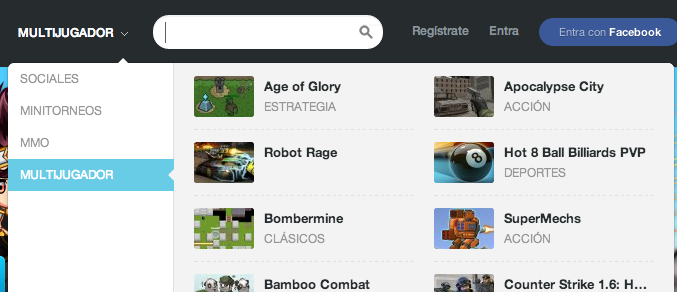
\includegraphics[width=\textwidth]{images/minijuegos-mul.png}
%%     \caption{Juegos multijugador en Minijuegos ({\tt http://www.minijuegos.com})}
%%     \label{fig::minijuegos-mul}
%%   \end{center}
%% \end{figure}

Un punto fuerte de Minijuegos es el conjunto de herramientas y recursos que ofrecen para el desarrollo de juegos por parte de terceros. Ponen \acs{API}s de diferentes tecnologías a disposición de los desarrolladores. Esto garantiza un éxito prolongado de la plataforma, dado que la sencillez de programación de juegos para la misma motiva a los desarrolladores a ampliar su catálogo cada día.

Los juegos están desarrollados en Flash (requieren la instalación de un plugin) y HTML5 (funcionan \acs{OOTB} con cualquier navegador moderno).

\subsection*{Miniclip.com}

Con el mismo pagerank\index{pagerank}, 6/10, Miniclip ofrece también una gran cantidad de juegos, clasificados en más de 70 categorías ---lo cual puede resultar algo abrumador para el usuario---. En la figura \ref{fig::miniclip} se muestra la parte de la interfaz de esta plataforma.

\begin{figure}
  \begin{center}
    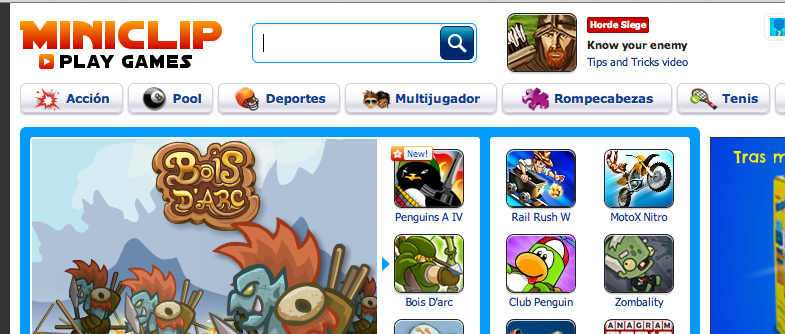
\includegraphics[width=\textwidth]{images/miniclip.png}
    \caption[Miniclip]{Miniclip$^{\ref{foot-miniclip}}$}
    \label{fig::miniclip}
  \end{center}
\end{figure}
\addtocounter{footnote}{1}\footnotetext{\label{foot-miniclip}{\tt http://www.miniclip.com}}

Visualmente, y en cuanto a usabilidad se refiere, Miniclip está muy por detrás de Minijuegos. Además se aprecian pequeños defectos, como el hecho de que exista una categoría llamada {\it Educación} y otra llamada {\it Educativos}, que dan una sensación de una menor profesionalidad.

Los juegos, tanto multijugador como individuales, están desarrollados en Flash y Unity, por lo que requieren la instalación de plugins para poder ser ejecutados.

\subsection*{Minigamesfreak.com}

Bajando bastante el nivel, tanto en cuanto a calidad de la plataforma como a pupularidad, se encuentra Minigamesfreak, con un pagerank\index{pagerank} de 2/10. Se trata de un sitio que recopila juegos individuales de otras plataformas, como Minijuegos. La usabilidad deja mucho que desear, teniendo que pasar por múltiples páginas desde que se hace click sobre un juego hasta llegar a él y poder jugar.

\begin{figure}[h]
  \begin{center}
    
\includegraphics[width=\textwidth]{images/minigamesfreak.png}
    \caption[Minigamesfreak]{Minigamesfreak$^{\ref{foot-minigamesfreak}}$}
    \label{fig::minigamesfreak}
  \end{center}
\end{figure}
\addtocounter{footnote}{1}\footnotetext{\label{foot-minigamesfreak}{\tt http://www.minigamesfreak.com}}
Minigamesfreak tiene un enfoque lucrativo mediante publicidad, algo abusiva, que produce una experiencia de usuario desagradable. Sin prestar ninguna atención al diseño ofrecen una apariencia deficiente y poco atractiva.

\subsection*{Juegosfan.com}

Al igual que Minigamesfreak, Juegosfan ofrece una recopilación de juegos (individuales o monojugador) de otras webs populares, como Minijuegos. No obstante, en este caso se trata de un sitio web más profesional y agradable para el usuario. Con un pagerank\index{pagerank} de 4/10 denota una popularidad importante en Internet.

\begin{figure}[h]
  \begin{center}
    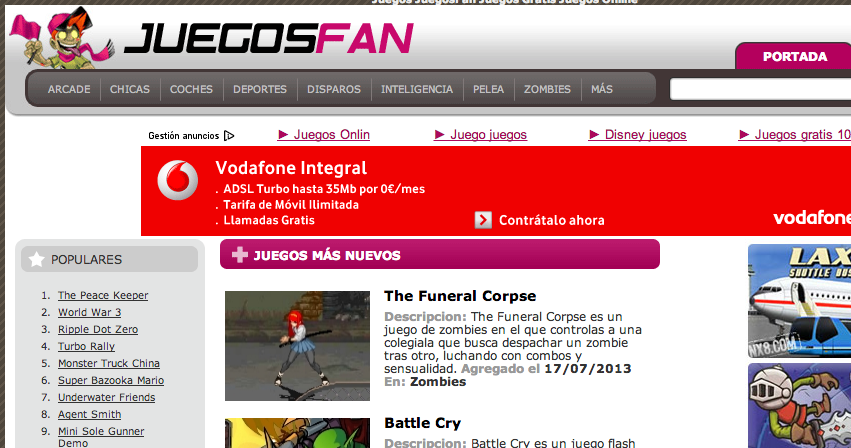
\includegraphics[width=\textwidth]{images/juegosfan.png}
    \caption[Juegosfan]{Juegosfan$^{\ref{foot-juegosfan}}$}
    \label{fig::juegosfan}
  \end{center}
\end{figure}

La interfaz que ofrece está un poco saturada de publicidad, por lo que la experiencia es mejorable.

\subsection*{Minigameonline.net}

De nuevo una web de recopilación de juegos de otras páginas, de un nivel de madurez y popularidad similar al de Minigamesfreak (pagerank\index{pagerank} de 2/10). Con una sencillez mayor, la experiencia de juego mejora frente al primero, dado que cargar cualquier juego es inmediato y no te obliga a pasar por páginas intermedias. Además la publicidad no resulta molesta y queda relegada a un segundo plano.

\begin{figure}[h]
  \begin{center}
    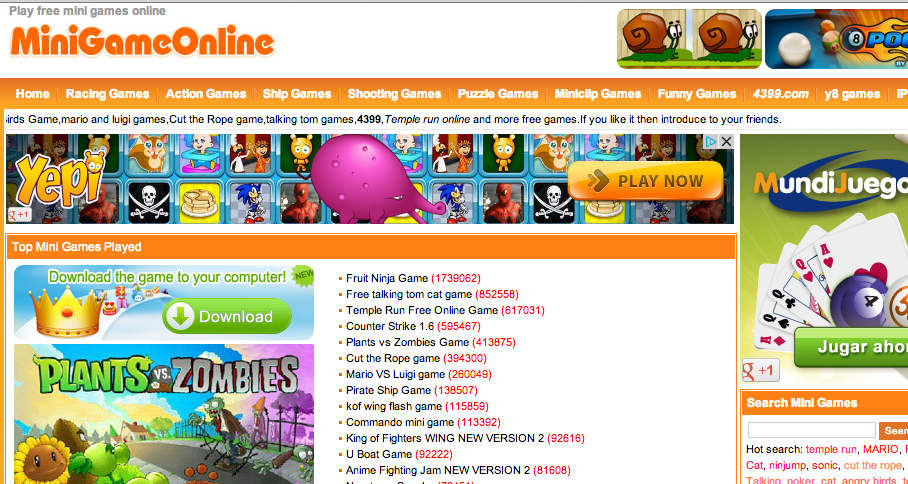
\includegraphics[width=\textwidth]{images/minigameonline.png}
    \caption[Minigameonline]{Minigameonline$^{\ref{foot-minigameonline}}$}
    \label{fig::minigameonline}
  \end{center}
\end{figure}

\addtocounter{footnote}{1}\footnotetext{\label{foot-juegosfan}{\tt http://www.juegosfan.com}}

Los juegos que integra están implementados en Flash, y clasificados en 8 categorías entre las que se incluyen, a parte de las clásicas (Carreras, Acción, Barcos, Disparos, Puzzle...), categorías específicas para las webs de las que se han extraído los juegos, como Miniclip.

\section{Entrenamiento cerebral mediante mini juegos}
\label{sec::webs-de-brain}

En las secciones anteriores han sido expuestas algunas de las plataformas de minijuegos más conocidas de Internet. Se trata de webs recopilatorias de juegos casuales de multitud de temáticas, donde los juegos enfocados al ingenio, la memoria o la educación juegan un papel poco importante ---indistinguible del de juegos de plataformas, carreras, acción, etc---.

En esta sección se analizarán otras plataformas de juegos, esta vez centradas en juegos de estimulación de habilidades mentales.

\subsection*{Lumosity.com}\index{lumosity}

Con un pagerank\index{pagerank} de 6/10, se trata de una de las webs más populares de minijuegos orientados a la estimulación de habilidades mentales. Muestra una interfaz sencilla, con un diseño muy agradable y sin publicidad. La ausencia de anuncios se agradece al utilizar la plataforma, pero tiene un gran inconveniente: el servicio ofrecido es de pago (ver figura \ref{fig::lumosity}). Las tarifas no son demasiado económicas, por lo que emplear la plataforma como entretenimiento casual queda totalmente descartado para la mayoría de usuarios. De forma gratuita no es posible probar ningún juego.
\addtocounter{footnote}{1}\footnotetext{\label{foot-minigameonline}{\tt http://www.minigameonline.net}}
Lumosity está enfocada sobre todo al entrenamiento rutinario, ofreciendo un seguimiento personalizado para cada usuario.

En esta plataforma los juegos son clasificados en 5 categorías: Velocidad, Memoria, Atención, Flexibilidad y Resolución de Problemas. Todos los juegos son individuales ---quedando así anulado cualquier atisbo ``social''--- y están implementados en Flash, con el inconveniente que ello supone: es necesario tener instalado un plugin para esta tecnología.

\begin{figure}[H]
  \begin{center}
    
\includegraphics[width=\textwidth]{images/lumosity.png}
    \caption[Lumosity]{Lumosity$^{\ref{foot-lumosity}}$}
    \label{fig::lumosity}
  \end{center}
\end{figure}
\addtocounter{footnote}{1}\footnotetext{\label{foot-lumosity}{\tt http://www.lumosity.com}}



\subsection*{Brainarena.com}

Con menor popularidad (pagerank de 3/10), Brainarena cambia el enfoque lucrativo hacia un modelo basado en la publicidad, ofreciendo sus servicios de forma totalmente gratuita (como ocurría con las plataformas estudiadas en la sección \ref{sec::webs-de-juegos}) a costa de empeorar considerablemente la experiencia de usuario.

Son sólo 16 juegos los que están al alcance del usuario. La ausencia de categorías para clasificarlos resulta un tanto extraña.

Por otro lado, la jugabilidad es sobresaliente debido a su sencillez: todos los juegos muestran una imagen y dan 4 opciones que pueden ser elegidas con las teclas 1, 2, 3 y 4 del teclado.

\section{Tecnologías Web}
\label{sec::desarrollo-web}

La imparable popularización de Internet ha sido propulsora de una gran evolución tecnológica y social desde que la {\it ``Red de redes''} fue concebida hasta nuestros días. Al principio de la década de los 90 tener un computador personal en casa era un lujo al alcance de pocos, y el acceso a Internet un lujo todavía mayor. Los teléfonos móviles no se empezarían a extender hasta 5 o 10 años después. A día de hoy cualquier persona tiene un ordenador en casa y acceso a Internet. Es más, según \cite{Accenture2012} el 69\% de los accesos a Internet en la actualidad se realizan desde teléfonos móviles.

\begin{figure}[H]
  \begin{center}
    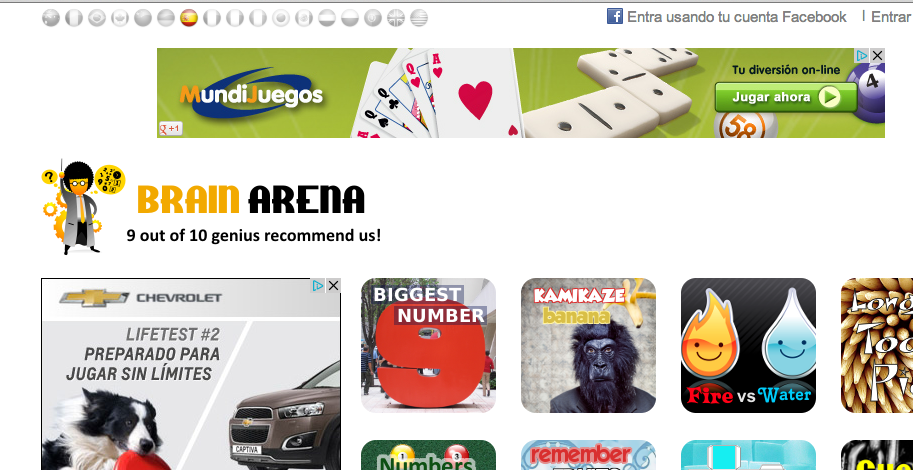
\includegraphics[width=\textwidth]{images/brainarena.png}
    \caption[Brainarena]{Brainarena$^{\ref{foot-brainarena}}$}
    \label{fig::brainarena}
  \end{center}
\end{figure}

\addtocounter{footnote}{1}\footnotetext{\label{foot-brainarena}{\tt http://www.brainarena.com}}


Internet es una red descentralizada de servicios como \acs{WWW}, \acs{SMTP}, \acs{FTP}, \acs{P2P}, \acs{IRC}, \acs{VoIP}, \acs{SSH}, etc. De entre ellos el de mayor éxito es el primero: la \acf{WWW}, conocida informalmente como {\it ``La Web''}. \acs{WWW} es un conjunto de protocolos que permite la consulta de archivos de hipertexto\index{hipertexto}\footnote{El hipertexto es una herramienta de software con estructura no secuencial que permite crear, agregar, enlazar y compartir información de diversas fuentes por medio de enlaces asociativos. El hipertexto es una de las formas de la {\it hipermedia}\index{hipermedia} ---manipulación de información interactiva en diversos formatos---.}.

La explicación más sencilla del funcionamiento de Internet consiste en la comprensión de dos conceptos: servidor y cliente. Los clientes envían peticiones al servidor, y éste construye y devuelve una respuesta. En el caso de la navegación web, la petición puede ser la solicitud \acs{HTTP}\index{HTTP} \acs{GET}\index{GET} de una página web, y la respuesta el código \acs{HTML}\index{HTML} de la web, que será interpretado y renderizado por el navegador del cliente. Otro ejemplo puede ser una petición \acs{HTTP}\index{HTTP} \acs{POST}\index{POST} de envío de un formulario, y una respuesta de redirección.

A continuación se presentan algunas de las tecnologías web más populares, tanto a nivel del servidor como del cliente.

\subsection{Servidor web}

Un servidor web es un computador que realiza, siguiendo un orden riguroso, las siguientes tareas:

\begin{enumerate}
\item Recibe una petición de un cliente
\item Procesa la petición
\item Realiza la tarea interna correspondiente a esa petición
\item Construye una respuesta
\item Envía la respuesta al cliente que hizo la solicitud
\end{enumerate}

En la actualidad existen numerosas tecnologías y entornos de ejecución para la construcción y despliegue de servidores web, en casi cualquier lenguaje de programación existente. Cada opción tiene sus ventajas e inconvenientes y es más o menos adecuada dependiendo de la situación y finalidad del servidor.

En el caso concreto de las páginas web, el servidor recibe peticiones \acs{GET} y \acs{POST} del navegador web de un cliente y genera código \acs{HTML} y de {\it scripting} (JavaScript) que dicho navegador es capaz de interpretar.

A continuación se exponen algunas de las tecnologías más utilizadas en la creación de servidores web.

\subsubsection{PHP}

PHP\index{PHP} es un lenguaje de {\it scripts} ---scripts del lado del servidor, por lo que no son interpretables por un navegador web cliente--- ampliamente utilizado para todo tipo de propósitos. Está orientado especialmente al desarrollo web, y puede ser empotrado en código \acs{HTML}\index{HTML} (ver listado \ref{code:php}).

\begin{listing}[language=html, caption={Ejemplo de inclusión de código PHP en HTML}, label=code:php]
<!DOCTYPE html>
<html lang="es">
    <head>
        <meta charset="UTF-8" />
        <title> Ejemplo basico PHP</title>
    </head>
    <body>
        <?php
            echo 'Esto es codigo PHP';
        ?>
    </body>
</html>
\end{listing}

Este lenguaje es software libre, y además de ser interpretado por un servidor web también permite su ejecución en un intérprete de comandos común. En \cite{php} se ofrecen recursos útiles para el aprendizaje y primeros pasos del lenguaje.

\subsubsection{ASP.NET}

A diferencia del anterior, éste es un framework diseñado exclusivamente para el desarrollo de páginas web dinámicas y servicios web. Es el sucesor del antiguo \acs{ASP}, lanzado por Microsoft en 1996. Permite su utilización con cualquier lenguaje soportado por el framework .NET (Java, C\#, etc.), y puede ser utilizado únicamente en servidores \acs{IIS} de Microsoft.

En comparación a otras alternativas interpretadas (como PHP), ASP.NET ofrece la ventaja de trabajar con código compilado, lo que le otorga mejor rendimiento.

\subsubsection{JSP (Java Server Pages)}

Aunque Java es un lenguaje de propósito general, no es hasta 1999 cuando Sun Microsystems lanza \acs{JSP} para competir con otros lenguajes y frameworks, PHP y \acs{ASP}.

Esta tecnología requiere una máquina virtual Java, capaz de interpretar su {\it bytecode} \index{bytecode}, y soporta lo que se conocen como anotaciones ---comentarios \acs{HTML} con una sintaxis especial, que permiten la modificación de ciertas partes del código en tiempo de ejecución---.

\subsubsection{NodeJS}

En los últimos años la popularización de JavaScript como lenguaje de programación web (del lado del cliente) ha crecido de forma considerable, ayudada en parte por el desarrollo del motor de ejecución V8 (creado por Google para el navegador Chrome). Lo que no se pensó hasta 2009 era en la posibilidad de utilizarlo en el lado del servidor. Fue entonces cuando Ryan Dahl lanzó NodeJS, un entorno de ejecución de JavaScript nativo, basado en el motor V8, centrado en la entrada salida y basado en eventos.

NodeJS es software libre, está enfocado a la escalabilidad y permite la creación de servidores web de manera realmente sencilla. El listado \ref{nodejs-example} muestra la implementación de un servidor \acs{HTTP} básico que responde ``Hello world''.

\begin{listing}[language=javascript, caption={Servidor web básico implementado con NodeJS}, label=nodejs-example]
var http = require('http');
 
http.createServer(function (request, response) {
    response.writeHead(200, {'Content-Type': 'text/plain'});
    response.end('Hello World\n');
}).listen(8000);
 
console.log('Server running at http://127.0.0.1:8000/');
\end{listing}

La popularidad de NodeJS resulta asombrosa, teniendo en cuenta que se trata de una tecnología muy nueva. En los cuatro años que lleva en desarrollo cuenta ya con más de 37000 módulos registrados en \acs{NPM}, lo que da una idea de la calurosa acogida que ha tenido por parte de la comunidad de desarrolladores.

\subsection{Cliente web}
\label{sec::desarrollo-juegos}

El cliente web es sencillamente un navegador corriente que, principalmente, accede a páginas web y realiza peticiones de formularios. Cuando un usuario accede a una página web, el navegador la solicita al servidor, éste la construye y la devuelve, y el navegador la interpreta y se la muestra al usuario.

Como veremos más adelante, la labor del navegador web va más allá de la mera petición e interpretación de páginas web. Concretamente cuando nos centramos en el desarrollo de videojuegos multijugador, el navegador es también el encargado de mantener la comunicación con el servidor de forma transparente al usuario.

\subsubsection{Tecnologías web para desarrollo de videojuegos}

Existen diversas tecnologías disponibles para la inserción de contenido gráfico animado e interactivo en una página web. A continuación se expondrán las más importantes, absolutas protagonistas del desarrollo de videojuegos web hoy en día.

\begin{itemize}

\item{\bf JApplets}

Durante un largo tiempo, los applets de Java (o JApplets) fueron la fuerza dominante en el desarrollo de contenido interactivo web en el lado del cliente. La popularización de Java como lenguaje de propósito general fue en gran parte la responsable. No obstante, con la modernización de \acs{HTML} y los navegadores web, muchas de las funcionalidades que antes se hacían mediante Java pasaron a estar soportadas \acs{OOTB}, por lo que esta tecnología de Java fue perdiendo popularidad. Nótese que los applets de Java requieren de un complemento adicional o plug-in instalado en el navegador para ser ejecutados.

En la actualidad se utiliza bastante poco, habiendo quedado prácticamente en desuso en el ámbito de los videojuegos (en parte por el bajo rendimiento gráfico que ofrece).

\item{\bf Flash y Shockwave}

Las tecnologías Flash y Shockwave, ambas desarrolladas por Macromedia (empresa que más adelante sería absorbida por Adobe), supusieron una gran evolución en el desarrollo de contenido interactivo web. Hoy en día son ampliamente utilizadas, y ofrecen un rendimiento muy bueno en la reproducción de contenido multimedia ---Shockwave soporta aceleración gráfica---.

Se trata de dos tecnologías complementarias, siendo Shockwave algo más amplia (es capaz de reproducir contenido Flash, lo que no ocurre a la inversa). Requieren de un plug-in para el navegador web. En el caso de Flash, el plug-in se encuentra en el 95\% de los computadores de escritorio, mientras que en el caso de Shockwave sólo en el 40\%, según \cite{w3techs}.

En la actualidad está ocurriendo algo similar a lo que pasó con los applets de Java, y es que \acs{HTML} y los navegadores modernos son capaces de llevar a cabo tareas que antes sólo podía hacer Flash, por lo que cada vez se está empezando a utilizar menos para algunas aplicaciones, debido en parte a la ventaja de no necesitar de plug-ins adicionales.

\item{\bf Unity web player}

Unity es un {\it ``ecosistema de desarrollo de videojuegos''}, según \cite{unity}. Bajo la filosofía \acf{WORE} permite el desarrollo de videojuegos compilables de forma automática para múltiples plataformas. El gran problema de Unity es que es de pago ---con un precio que oscila entre los 1500 y los 6500 euros---, por lo que no se encuentra al alcance de todos los bolsillos.

Entre las ventajas que ofrece frente a otras alternativas, las más importantes son:
\begin{itemize}
\item Rendimiento
\item Calidad gráfica
\item Soporte de plug-ins
\end{itemize}
Unity web player es el componente que permite la ejecución en un navegador de videojuegos creados con Unity. Tal y como ocurría con Flash y Shockwave, si el navegador web no cuenta con el plugin instalado no será capaz de ejecutar el componente.

\item{\bf HTML5}
  
El lenguaje de marcado \acs{HTML} ha ido adaptándose a las necesidades surgidas a causa de la evolución de Internet. En este sentido, la especificación de la última versión (aún no cerrada por completo) incluye funcionalidades que antes eran propias de Flash o los applets de Java, y que ahora cualquier navegador web moderno es capaz de desempeñar. Buen ejemplo de estas funcionalidades son la inclusión de audio y vídeo, así como el objeto {\tt canvas}, que posibilita la creación de videojuegos complejos con un renidmiento excelente.

La tecnología WebGL, parte de la especificación de HTML5, permite incluso utilizar la aceleración gráfica para reproducir contenido 3D de alta calidad. No es de extrañar que HTML5 esté acabando poco a poco con otras tecnologías (que requieren complementos adicionales para ser ejecutadas).

En la figura \ref{fig::webgl} se muestra un ejemplo de la calidad gráfica ofrecida por HTML5. En \cite{chrome-experiments} existe un gran surtido de ejemplos para experimentar con este tipo de contenidos web.

\end{itemize}

\begin{figure}[h]
  \begin{center}
    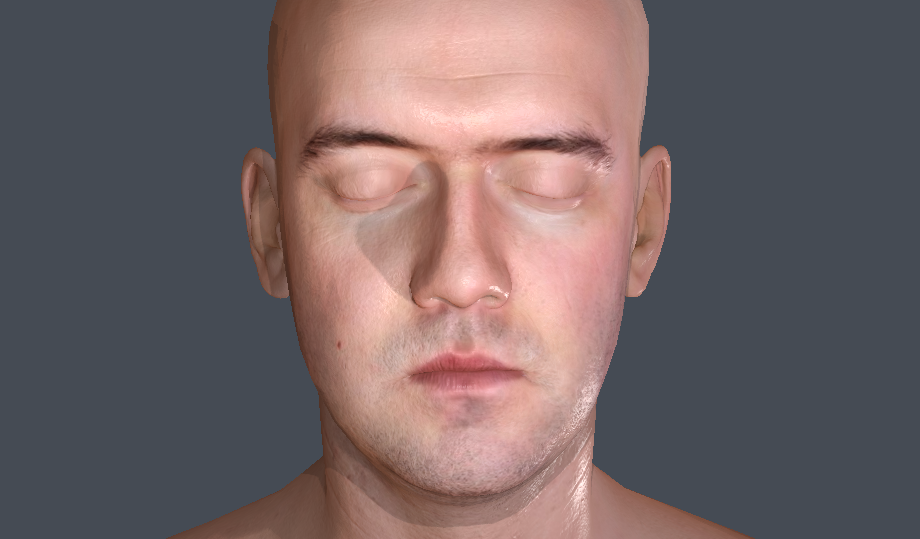
\includegraphics[width=\textwidth]{images/webgl.png}
    \caption{Muestra de las posibilidades gráficas de HTML5 con WebGL}
    \label{fig::webgl}
  \end{center}
\end{figure}

\subsubsection{Comunicación web ininterrumpida: websockets}
\label{sec::tiempo-real}

WebSocket es una tecnología que implementa sockets de comunicación entre servidores y navegadores web (aunque pueden utilizarse por cualquier tipo de aplicación cliente/servidor). Proporciona un canal de comunicación bidireccional y full-duplex sobre un único socket TCP.

Se trata de una tecnología que aún se encuentra en desarrollo. La API de WebSocket está siendo normalizada por el W3C, y el protocolo WebSocket, a su vez, está siendo normalizado por el IETF.

Como las conexiones TCP ordinarias sobre puertos diferentes al 80 suelen ser bloqueadas por los administradores de redes, el uso de esta tecnología proporcionaría una solución mediante la multiplexación de diferentes servicios WebSocket sobre un único puerto TCP.

La especificación del protocolo WebSocket define dos nuevos esquemas de URI:

\begin{itemize}
\item {\tt wss:} para conexiones cifradas
\item {\tt ws:} para conexiones no cifradas
\end{itemize}

El resto de componentes del URI se definen con la sintaxis genérica de URI.

\section{Anatomía y fisiología del cerebro humano}
\label{sec::fisiologia}

% http://www.lumosity.com/knowledge-center/brain-reference/

El primer paso antes de tratar de emplear conocimientos técnicos para mejorar las habilidades mentales de los seres humanos es, evidentemente, la familiarización con la fisiología\footnote{Ciencia biológica que estudia las funciones de los seres orgánicos.} del cerebro, pues de nada sirve tratar de mejorar algo sin conocerlo previamente. En este sentido se ha realizado un esfuerzo adicional por ofrecer esta base científica de una forma amena para el lector. Así pues, en las siguientes secciones se realizará un recorrido por los aspectos más relevantes en cuanto a la estructura y funcionamiento del {\it ``órgano más importante de todos''} \cite{Jacyna2009}.

Una vez adquiridos esos conocimientos previos sobre la materia, nos encontraremos en disposición de diseñar e implementar los mecanismos y métricas más adecuados para la mejora de las funciones cerebrales humanas.

\subsection{Estructura cerebral}

El cerebro de una persona viva es de color rosa, algo pálido. {\it ``Conservado en formol, el cerebro endurece y pierde su color''}, afirma \cite{Czerner2001}. En esta sección hablaremos de las células que constituyen la estructura el cerebro. Estas células se organizan en dos grupos:


\begin{itemize}
\item núcleo\index{núcleo}
\item corteza (o {\it córtex}\footnote{A lo largo de este texto se emplearán indistintamente los términos \emph{corteza} y \emph{córtex}, dado que así se hace en la literatura médica en nuestro idioma.})\index{córtex}
\end{itemize}


\subsubsection{Materia gris, materia blanca y células gliales}

El cerebro es en gran parte de color gris, y es por ello que se emplea la denominación {\it materia gris}. La materia gris está formada por miles de millones de neuronas. Tiene la {\it ``consistencia blanda de harina de avena cocida''}, afirma \cite{Czerner2001}. En la figura \ref{diagrama_neurona} puede apreciarse la forma general de una neurona.


\begin{figure}[h]
  \begin{center}
    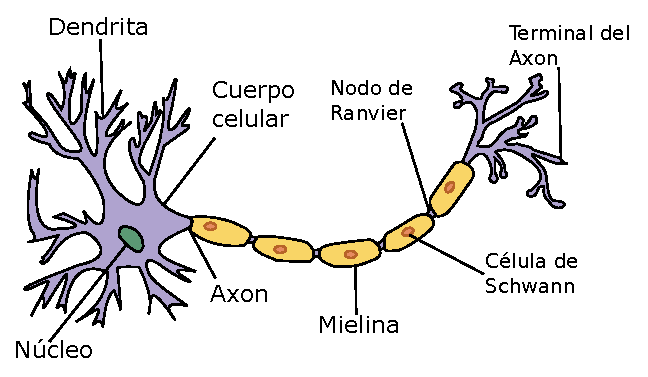
\includegraphics[scale=1]{images/neurona.eps}
    %http://upload.wikimedia.org/wikipedia/commons/6/62/Neurona.svg
    \caption{Diagrama sencillo de una neurona}
    \label{diagrama_neurona}
  \end{center}
\end{figure}


Puesto que hay tantas neuronas, es tentador considerarlas diminutas en términos de su alcance, pero en realidad algunas neuronas tienen axones muy largos. Cuando una multitud de axones se agrupan, aparecen como {\it materia blanca}. En \cite{Czerner2001} se describe la materia blanca como {\it ``una colección de axones largos, aislados, ramas salientes de neuronas que conectan las diversas partes del cerebro entre sí''}, debiendo el color blanco a {\it ``la mielina, un reluciente material aislante que envuelve los largos axones''}.

\cite{Damasio1994} proporciona una descripción sucinta de las materias blanca y gris: {\it ``La materia gris corresponde en gran parte a las colecciones de cuerpos de células nerviosas, mientras que la materia blanca corresponde en gran parte a los axones, o fibras nerviosas, que emanan de los cuerpos celulares en la materia gris''}. Las neuronas se encuentran {\it ``apoyadas por las células gliales''}, que son {\it ``esenciales para la actividad del cerebro''}

Por otro lado, en \cite{Czerner2001} encontramos una buena descripción de las células gliales: {\it ``Cada neurona está rodeado por entre diez y cincuenta células gliales, que constituyen la mayor parte del cerebro. Las células gliales apoyan a la neurona de varias maneras: proporcionan el soporte estructural, aíslan las ramas neuronales con mielina para acelerar la transmisión de señales eléctricas por su axones, mantienen la nutrición de la neurona, ayudan en la eliminación de residuos, e incluso establecen los marcadores que conducen las ramas de una neurona en desarrollo a su destino correcto''}. Como detalle curioso, en el mismo libro se afirma que {\it ``un estudio del cerebro de Albert Einstein demostró que es posible que tuviera un exceso de células gliales''}.

\subsubsection{Cortezas y núcleos cerebrales}

{\it ``La materia gris se presenta en dos variedades''}, afirma \cite{Damasio1994}. {\it ``La primera variedad de materia gris es la formada neuronas que se colocan en capas, como en una torta, para formar una corteza. Ejemplos son la corteza cerebral que cubre los hemisferios cerebrales y la corteza cerebelosa que envuelve el cerebelo. En la segunda variedad de materia gris, las neuronas no están estratificadas, sino que se organizan como cacahuetes dentro de un tarro de cristal. Esta formación constituye un núcleo''}.

\index{neocórtex}

El mejor ejemplo de neuronas organizadas en forma de corteza es la {\it neocorteza} o {\it neocórtex}, a menudo llamada {\it corteza cerebral}. El neocórtex se pliega de una manera que permite a una superficie más grande encajar dentro de los confines del cráneo humano. Los anatomistas llamar {\it surcos} a los pliegues corticales, y {\it giro} a la zona lisa entre dichos pliegues. En la figura \ref{surcosygiros} pueden apreciarse tanto los surcos como los giros de la corteza cerebral.

\begin{figure}[h]
  \begin{center}
    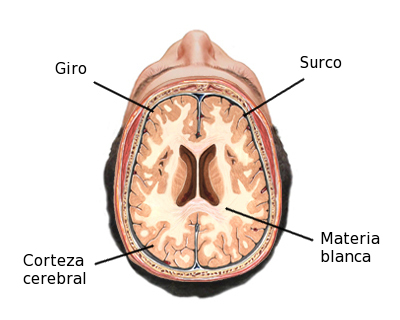
\includegraphics[scale=0.8]{images/surcosygiros.jpg}
    %http://nymethodist.adam.com/graphics/images/en/19238.jpg
    \caption{Surcos y giros del cerebro humano}
    \label{surcosygiros}
  \end{center}
\end{figure}

\subsubsection{Las neuronas}

Los componentes principales de una neurona se detallan en la figura \ref{diagrama_neurona}. La longitud del axón puede ser mucho más larga de como se muestra en la ilustración, tal y como ya se ha dicho cuando se han introducido los conceptos de {\it materia gris} y {\it materia blanca}. Asimismo, en \cite{Sapolsky} se resalta la complejidad de una sola neurona, explicando que puede tener una media de 10.000 dendritas y 10.000 terminales de axón. La comunicación entre las neuronas es tanto química como eléctrica, así que el término electroquímica se utiliza para describir el proceso global.

Simplificando mucho, las moléculas químicas llamadas \index{neurotransmisor} {\it neurotransmisores} son las encargadas de llevar mensajes de una neurona a otra consecutiva. Las vesículas en las terminales del axón de una neurona liberan moléculas de neurotransmisores. Desde un punto de vista químico, una molécula de neurotransmisor {\it ``se ajusta como una llave en una cerradura''}, dice \cite{Sapolsky}, cuando hace contacto con un receptor en las dendritas de una segunda neurona. En \cite{Restak1995} se explica que {\it ``Los receptores son grandes moléculas de proteínas dinámicos que se encuentran a lo largo y dentro de la membrana celular''}. Los receptores pueden, explica el texto, {\it ``verse aumentadas en número y avidez por su neurotransmisor según las circunstancias. Grandes y prolongadas ingestas de ciertas sustancias, por ejemplo, llevar a un aumento en el número de receptores para estas sustancias ---esta es la base de la adicción a las drogas---... Más tarde, si la persona adicta se mantiene alejada de las drogas, los receptores pueden morir''.}

La unión del neurotransmisor y receptor es inhibidora o excitadora. {\it ``Cada neurotransmisor influye en su propio receptor independiente de la acción de los receptores de otros''}, dice \cite{Restak1995}. {\it ``Si bien algunos neurotransmisores pueden disminuir la tensión entre el interior y el exterior de la célula nerviosa y así estimular la célula en acción (neurotransmisor excitador), otras lo aumentan y por lo tanto inhiben la célula de cocción (neurotransmisor inhibidor''}.

Una vez que el \index{neurotransmisor} neurotransmisor y receptor se unen entre sí, \cite{Restak1995} describe su acción como ``dinámica'' y ``exquisitamente sensible''. Hay dos familias de receptores: 

\begin{itemize}

\item {\bf Receptores de canal iónico}

Provocan cambios en la permeabilidad de la membrana y, por lo tanto, regulan el flujo de iones a través de su canal. Cuando un \index{neurotransmisor} neurotransmisor reacciona con su receptor, produce como resultado un cambio en la forma del receptor, de modo que los iones pueden entonces fluir a través de la membrana desde el punto de alta concentración hacia el punto de menor concentración.

\item {\bf Receptores sin canales iónicos}

Actúan a través de intermediarios, las proteínas G, ubicadas en el interior de la célula nerviosa. Básicamente, las proteínas G funcionan como factores de acoplamiento que sirven como enlaces entre el receptor de la superficie exterior de la membrana de la célula nerviosa y un gran número de procesos celulares relacionados entre sí dentro de la célula.

\end{itemize}

Una excitación suficiente en los receptores de los canales iónicos de las espinas dendríticas provoca una onda de cambio iónico que lleva al axón de la neurona a alcanzar su máximo potencial de acción. Una señal eléctrica así desplaza hacia abajo el axón de la neurona y los terminales de los axones para provocar que las vesículas liberen un neurotransmisor químico. En otras palabras, la neurona ``dispara''. Como las vesículas liberan moléculas neurotransmisoras, cada molécula queda ``a la deriva'', con el potencial de hacer contacto con un receptor. Las neuronas, comunicándose entre sí en una dirección, producen un circuito. A menudo existen circuitos alternativos entre las mismas estructuras cerebrales.

Los circuitos neuronales locales en el neocórtex constituyen regiones corticales. Las regiones corticales no solo pueden conectarse unas con otras, sino también con los núcleos subcorticales.

\subsubsection{Neuronas, proyecciones y vías}

\cite{Damasio1994} explica que {\it ``un haz de axones provenientes de fuente conocida y hacia un objetivo determinado se conoce a menudo como proyección, porque proyecta axones a una colección de neuronas. Una secuencia de proyecciones a través de varias estaciones de destino se conoce como vía''}. A menudo se puede ver una vía (materia blanca) a simple vista. Como se ha mencionado antes, \cite{Czerner2001} describe la materia blanca como {\it ``una colección de axones largos, aislados, ramas salientes de neuronas que conectan las diversas partes del cerebro entre sí''}.

% \subsection{El ADN y el comportamiento humano}

% \cite{Brockman} escribe: {\it ``Un gen es un paquete de información, no un objeto o cosa. El patrón de pares de bases en una molécula de ADN especifica el gen, pero la molécula de ADN... es el medio, no el mensaje. Mantener esta distinción entre el medio y el mensaje es absolutamente indispensable para la claridad de pensamiento acerca de la evolución''}.

% A modo de introducción a la genética, hagamos un repaso de abajo a arriba: Existen cuatro compuestos básicos (llamados bases): {\it Citosina}, {\it Adenina}, {\it Timina}, y {\it Guanina}. Estos compuestos se unen entre sí en pares de bases (ver figura \ref{bases}):

% \begin{itemize}
% \item La Adenina (A) se empareja con la Timina (T).
% \item La Citosina (C) se empareja con la Guanina (G). 
% \end{itemize}

% \begin{figure}[h]
%   \begin{center}
%     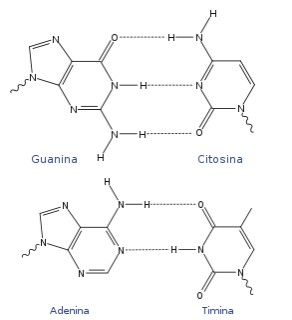
\includegraphics[scale=0.8]{images/bases.jpg}
%     % http://www.forcesystem.com.br/wp-content/uploads/2010/05/adenina-timina-gaunina-citosina.jpg
%     \caption{Pares AT y GC}
%     \label{bases}
%   \end{center}
% \end{figure}

% Estos pares de bases se conectan entre sí para formar dos hélices emparejados, conocidos como {\it ácido desoxirribonucleico (ADN)}. En \cite{JohnAllman2000} se explica cómo se lee el código de pares de bases:

% \begin{quote}
% {\it ``El código de pares de bases se lee en una dirección a lo largo de una hebra. Las secuencias de tres letras (tripletes), especifican cada aminoácido, y las secuencia de tripletes a su vez, especifican la cadena de aminoácidos que forma una proteína. Hay 64 posibles secuencias de tripletes, cada uno codifica uno de los 20 aminoácidos. Así, algunos aminoácidos son especificados por más de un triplete. Los otros tres tripletes son signos de parada que señalan el final de una proteína en concreto. La secuencia completa de tripletes que codifica una proteína es un gen''}.
% \end{quote}

\subsection{El desarrollo cerebral}

Es momento de estudiar el proceso de formación del cerebro humano.


\subsubsection{Introducción a la embriología}
\index{capas germinales}\index{embriología}
En \cite{Shubin2009} se ofrece una genial introducción a lo que se conoce como {\it capas germinales} y a la embriología:


\begin{quote}
{\it ``En la década de 1800, algunos filósofos naturales estudiaron a los embriones para tratar de encontrar el plan común para la vida en la tierra. Uno de estos observadores fue Karl Ernst von Baer, nacido en una familia noble, que inicialmente se formó para ser médico. Su mentor académico sugirió que para tratar de entender cómo funcionan los órganos de un pollo desarrollado, debía estudiar y entender el desarrollo del pollo.

Desafortunadamente, von Baer no podía permitirse el lujo de trabajar en incubadoras de pollos, ni podía permitirse muchos huevos. Por suerte para él, tenía un amigo rico, Christian Pander, que podía darse el lujo de hacer los experimentos. Mientras se fijaban en los embriones, se encontraron con algo fundamental: todos los órganos del pollo se puede remontar a una de las tres capas de tejido del embrión en desarrollo. Estas tres capas se conocían como las capas germinales. Lograron un estatus casi legendario, que conservan aún hoy en día.

El descubrimiento de las tres capas de von Baer dio los medios para hacer preguntas importantes: ¿Todos los animales comparten este patrón? Son el corazón, los pulmones y los músculos de los animales derivados de estas capas? Y, sobre todo, ¿las mismas capas se convierten en los mismos órganos en especies diferentes?

Von Baer comparó las tres capas de embriones de pollo con todo lo demás que pasara por sus manos: peces, reptiles y mamíferos. Efectivamente, pudo concluir que todos y cada uno de los órganos animales se habían originado en una de estas tres capas. Significativamente, las tres capas se formaron con las mismas estructuras en todas las especies. Cada corazón de cada especie estaba formado a partir de la misma capa. Otra capa daba lugar al cerebro de los animales. Y así sucesivamente. No importa lo diferentes que sean las especies, tanto adultos como pequeños embriones, todos pasamos por las mismas etapas de desarrollo''.}

\end{quote}

\subsubsection{Tubo neural}
\label{tubo}
El cerebro comienza a formarse a partir de una estructura en forma de tubo que se conoce como {\it tubo neural}. \cite{Lautin2001} afirma que el comienzo de todo el sistema nervioso central puede ser concebido como un globo inflado, alargado como el que usan los payasos para hacer globoflexia. El tubo neural se flexiona en dos puntos: la {\it flexión cervical} y la {\it flexión cefálica}.

\index{prosencéfalo}\index{mesencéfalo}\index{rombencéfalo}
En las primeras etapas del desarrollo humano, sólo hay tres bultos o vesículas en el tubo neural. A medida que se desarrolla el embrión, estas vesículas comienzan a diferenciarse en subdivisiones que se denominan comúnmente {\it prosencéfalo}, {\it mesencéfalo} y {\it rombencéfalo}. Los seres humanos comparten estas características de desarrollo en el cerebro con todos los demás vertebrados, incluidos los peces vertebrados, los anfibios, los reptiles, las aves y, por supuesto, otros mamíferos.


\begin{figure}[h]
  \begin{center}
    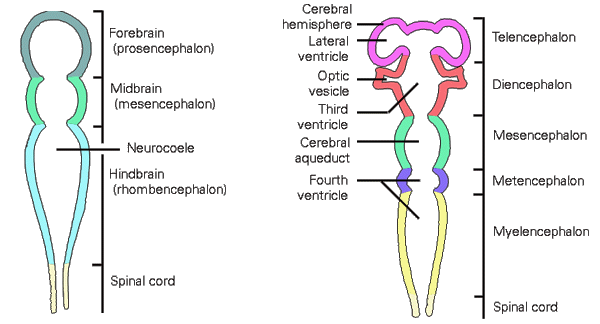
\includegraphics[width=\textwidth]{images/tubo-neural.png}
    % http://www.uoguelph.ca/zoology/devobio/210labs/neuraldevel1.html
    \caption{Tubo neural. A la izquierda el aspecto del tubo en la etapa más temprana de desarrollo, donde pueden apreciarse las 3 partes principales: prosencéfalo, mesencéfalo y rombencéfalo. A la derecha, en una etapa posterior, el prosencéfalo ha pasado a formar el telencéfalo y el diencéfalo.}
    \label{tubo-neural}
  \end{center}
\end{figure}

La figura \ref{tubo-neural} muestra el comienzo de la división del tubo neural. \cite{Lautin2001} señala que, debido a que todo se coloca inicialmente en la línea media, los ventrículos laterales ---una cavidad interna de los hemisferios cerebrales, que serán estudiados en la sección \ref{sec:hemisferios}--- tienen que ser divisiones laterales en los que el tubo neural se vuelve hacia el exterior. En la figura \ref{tubo-neural} se puede apreciar cómo esas divisiones del prosencéfalo comienzan a tomar forma para producir el {\it telencéfalo} (que después evoluciona y forma los hemisferios cerebrales) y el {\it diencéfalo} (que pasa a formar el {\it tálamo} y el {\it hipotálamo}).
\index{telencéfalo}\index{diencéfalo}\index{tálamo}\index{hipotálamo}

En \cite{Lautin2001} se explica que el telencéfalo es ``el ventŕiculo más evolucionado'', una especie de ``cerebro bien formado''. El prefijo {\it tele}, del griego antiguo, significa ``a distancia''. Por otro lado, el prefijo {\it di} de {\it diencéfalo}, según \cite{Lautin2001}, se explica porque el diencéfalo es una especie de ``cerebro de en medio'' o ``inter-cerebro''.


Si bien el \index{mesencéfalo} {\it mesencéfalo} permanece relativamente indiferenciado, el \index{rombencéfalo} {\it rombencéfalo} pasa a formar dos vesículas: la {\it metencéfalo} \index{metencéfalo} (que después pasa a formar el {\it puente troncoencefálico} (o protuberancia anular) y el {\it cerebelo}) y el \index{mielencéfalo} {\it mielencéfalo} (que después se convierte en el {\it bulbo raquídeo}). \index{bulbo raquídeo} \index{puente troncoencefálico} \index{protuberancia anular}

\subsubsection{Integración de neurocircuitos}

A medida que el cerebro se desarrolla, los circuitos neuronales son creados para integrar el cerebro en un todo funcional. \cite{Damasio1994} deja esto claro: {\it ``Hay miles de millones de neuronas en los circuitos de un cerebro humano, el número de sinapsis que se forman entre ellas es al menos de 10 billones, y la longitud de los axones de las neuronas que forman el cableado de los circuitos asciende al orden de cientos de miles de millas. La escala de tiempo para la transferencia de información es muy pequeña, del orden de decenas de milisegundos, lo que significa que en un segundo en la vida de la mente, el cerebro produce millones de patrones de activación sobre una gran variedad de circuitos distribuidos en varias regiones del cerebro''}. Más tarde, el autor añade: {\it ``Los secretos elementales de la mente residen, local y globalmente, en el momento de la interacción neuronal al disparar patrones generados por los circuitos neuronales del cerebro de un organismo vivo''}.

Los desequilibrios en la neurotransmisión de los circuitos cerebrales causan síntomas tales como obsesiones, compulsiones, tics nerviosos y déficit de atención. Algunos factores que influyen en estos desequilibrios son las infecciones virales o bacterianas, incesantes formas de estrés, lesiones físicas, la vulnerabilidad genética, o una combinación de factores. \cite{Damasio1994} afirma que {\it ``La distinción entre enfermedades del cerebro (mente), problemas neurológicos, y problemas psicológicos o psiquiátricos es una desafortunada herencia cultural que permanece en la sociedad, y la medicina refleja una ignorancia básica de la relación entre el cerebro y la mente''}.

\subsection{Estructuras primarias del cerebro}
\label{sec::estructuras-primarias}

{\it ``Debajo de la corteza cerebral, el cerebro humano tiene un parecido sorprendente con los de otras especies mucho más antiguas''}, explica \cite{Czerner2001}. Así como lo hacen en la mayoría de los animales, las neuronas del el bulbo raquídeo y el puente troncoencefálico situado en la base del cerebro, donde nace la médula espinal, de manera constante y fiable regulan sus funciones vegetativas, automatizando su actividad corporal como los latidos del corazón y la respiración. \index{puente troncoencefálico}

\subsubsection{El tronco encefálico. La formación reticular}

El denominado {\it tronco encefálico} (o {\it tallo cerebral}) incluye el \index{mesencéfalo} {\it mesencéfalo} o cerebro medio, \index{puente troncoencefálico} el {\it puente troncoencefálico} y el {\it bulbo raquídeo}. El núcleo del tallo cerebral se llama {\it formación reticular}. La palabra {``reticular''} significa {``red como''}, por lo que dicho núcleo describe el aspecto estructural del tejido del tallo cerebral. Por otro lado, el {\it sistema de activación reticular}, como puede leerse en \cite{Lindberg.}, es {\it ``una parte de la formación reticular que se extiende desde el tronco cerebral hasta el mesencéfalo y el tálamo, con conexiones distribuidas por toda la corteza cerebral y que controla el grado de actividad del sistema nervioso central ---por ejemplo, mantiene el sueño y la vigilia, así como la transición entre los dos estados''}. Existen diversos neurotransmisores implicados en la función reticular del sistema de activación, como la {\it acetilcolina} y \index{acetilcolina}\index{norepinefrina} la {\it norepinefrina}. 

Las neuronas encargadas de la segregación de {\it serotonina}, llamadas \index{núcleos del rafé} {\it núcleos del rafé}, forman una cresta o costura en el centro de la formación reticular. \cite{Panksepp1998} explica que estas neuronas están {\it ``situadas en la línea media del cerebro, lo que indica que son muy antiguas en la evolución del órgano''}. 

En \cite{JohnAllman2000} se señala que {\it ``la red de neuronas serotoninérgicas en el tronco cerebral estaba presente en los primeros vertebrados y ha mantenido una posición anatómica notablemente constante durante la evolución de vertebrados. Las neuronas serotoninérgicas se llaman así porque segregan, desde sus terminales de axón, el neurotransmisor llamado serotonina''}. Más adelante continúa: {\it ``los cuerpos celulares de las neuronas serotoninérgicas ocupan prácticamente la misma ubicación en el interior de cada cerebro de los vertebrados y se encuentran incluso en el mismo lugar en el sistema nervioso central. Este sistema ha sido increíblemente conservado durante la evolución, sin embargo, participa vitalmente en los aspectos más complejos de nuestro pensamiento y de las emociones''}. 

\subsubsection{Generación de patrones}

Aunque rara vez nos detengamos a pensar en ello, nuestro cerebro constantemente genera patrones de actividad, aparentemente sin esfuerzo. Muchos de estos patrones puede continuar incluso después de que ``se apague'' la conciencia. El {\it tallo cerebral} es el ejemplo más obvio de un generador de patrones. En \cite{Shubin2009} se explica lo siguiente: {\it ``Nuestro cerebro puede controlar nuestra respiración sin ningún esfuerzo consciente por nuestra parte. La mayor parte de ese trabajo se lleva a cabo en el tronco cerebral, en el límite entre el cerebro y la médula espinal. El cerebro envía impulsos nerviosos a los músculos respiratorios principales. La respiración sigue un patrón en el que están implicados los músculos del pecho, el diafragma y la garganta, trabajando en un orden bien definido. Por consiguiente, esta parte del tallo cerebral se considera un }generador central de patrones. {\it Esta región puede producir patrones rítmicos nerviosos y, en consecuencia, la activación de los músculos correspondientes. Un número de generadores de este tipo en el cerebro y la médula espinal se encargan del control de otros comportamientos rítmicos, como la ingesta y el caminar''}.

\subsubsection{El sistema nervioso autónomo (SNA)}

Según \cite{Sapolsky2004} "la manera principal en que el cerebro puede decirle al resto del cuerpo lo que debe hacer es el envío de mensajes a través de los nervios que se ramifican desde el cerebro hasta la columna vertebral y hacia la periferia de su cuerpo''. Conocemos mucho el sistema nervioso voluntario, donde {\it ``tú decides mover un músculo y lo mueves''}, dice el autor. Él explica que existe otra parte del sistema nervioso, el {\it sistema nervioso autónomo (\acs{SNA})}, que controla los eventos más espontáneos e involuntarios, tales como el rubor, la {\it piel de gallina}, y el orgasmo.

\cite{Lindberg.} define el SNA como {\it ``una parte del sistema nervioso de los vertebrados que regula las acciones involuntarias''}. Por otro lado, según \cite{MerckCo.} el sistema nervioso autónomo {\it ``funciona automáticamente (de manera autónoma), sin esfuerzo consciente de una persona''} y {\it ``controla los órganos internos, incluyendo los vasos sanguíneos, el estómago, el intestino, el hígado, los riñones, la vejiga, los genitales, los pulmones, los músculos de los ojos, el corazón y el sudor, la saliva y las glándulas digestivas''}.

El \acs{SNA} se compone de dos subsistemas: el {\it sistema nervioso parasimpático} y el {\it sistema nervioso simpático}. La función del sistema nervioso parasimpático es promover la calma, con funciones tales como el descanso y la digestión, mientras que la función del sistema nervioso simpático es la de preparar al indivíduo para luchar o huir. En la figura \ref{fig:sna} se muestra una panorámica fácil de recordar de esta división funcional.

\begin{figure}[h]
  \begin{center}
    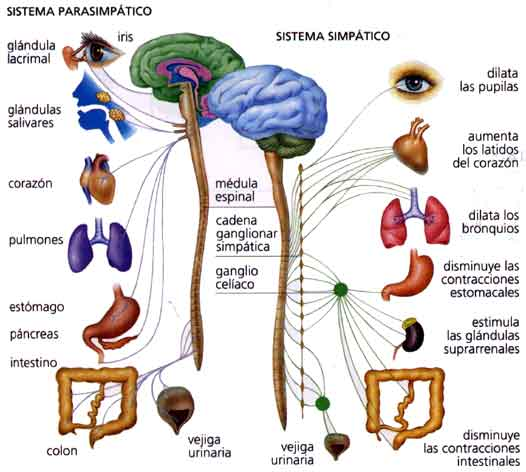
\includegraphics[scale=0.7]{images/sna.jpg}
    % http://lalupa3.webcindario.com/biologia/imagenes/simpatico%20y%20parasimpatico.jpg
    \caption{Subsistemas simpático y parasimpático del SNA}
    \label{fig:sna}
  \end{center}
\end{figure}

\subsubsection{El cerebelo}

\cite{Lindberg.} destaca que el {\it cerebelo} \index{cerebelo} (del latín ``pequeño cerebro'') está {\it ``situado entre el tronco cerebral y la parte posterior del cerebro en los seres humanos, y formado por dos lóbulos laterales y un lóbulo medio''}. En la figura \ref{fig:cerebelo} puede apreciarse la localización del mismo. 


\begin{figure}[h]
  \begin{center}
    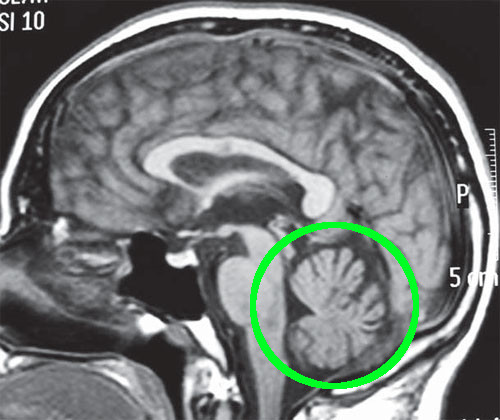
\includegraphics[scale=0.4]{images/cerebelo.jpg}
    % http://www.scielo.cl/fbpe/img/rchnp/v47n3/art07-3.jpg
    \caption{Localización del cerebelo}
    \label{fig:cerebelo}
  \end{center}
\end{figure}

La función principal del cerebelo es la de integrar las vías sensitivas y las vías motoras. Existe una gran cantidad de haces nerviosos que conectan el cerebelo con otras estructuras encefálicas y con la médula espinal. El cerebelo integra toda la información recibida para precisar y controlar las órdenes que la corteza cerebral manda al aparato locomotor a través de las vías motoras. Por ello, lesiones a nivel del cerebelo no suelen causar parálisis pero sí desordenes relacionados con la ejecución de movimientos precisos, mantenimiento del equilibrio, la postura y aprendizaje motor.

Como último detalle, de acuerdo con \cite{MerckCo.} {\it ``hay un creciente consenso en que, además de la coordinación, el cerebelo controla algunos aspectos de la memoria, el aprendizaje y la cognición''}. El texto explica que, aunque la \index{ataxia} {\it ataxia} --- una enfermedad que se caracteriza por provocar la descoordinación en el movimiento de las partes del cuerpo--- es el síntoma más típico de disfunción cerebelosa, muchas otras anomalías motoras también pueden ser fruto de esta disfunción.



\subsection{Los hemisferios cerebrales}
\label{sec:hemisferios}
El cerebro se divide en dos mitades prácticamente simétricas denominadas {\it hemisferios cerebrales} (figura \ref{hemisferios}). En \cite{Restak1994} se analiza cómo los hemisferios izquierdo y derecho responden ante diferentes situaciones, para determinar la funcionalidad de cada uno:

\begin{quote}
{\it ``El hemisferio derecho es dominante para cuestiones no verbales, tareas espaciales, interpretación de gestos faciales y emociones, visualización y transformación mental, y para la apreciación e intuición de figuras geométricas. Por otro lado, el hemisferio izquierdo se centra en el habla, la escritura y la comprensión oral, así como el cálculo.\\
Pero aún más importante que la división funcional es el hecho de que cada hemisferio tiene su propia consciencia.''}
\end{quote}

Ambos hemisferios funcionan de forma diferente al procesar emociones. Mientras que el hemisferio derecho responde ante emociones negativas, el izquierdo lo hace ante emociones positivas. Cuando el hemisferio derecho sufre daños, en \cite{Panksepp1998} se explica que {\it ``con frecuencia los pacientes permanecen alegres, pese a la gravedad de sus problemas''}. Por otro lado, un daño similar en el hemisferio izquierdo {\it ``puede causar estrés emocional catastrófico, predisponiendo a los pacientes a sufrir depresión''}.

\begin{figure}[h]
  \begin{center}
    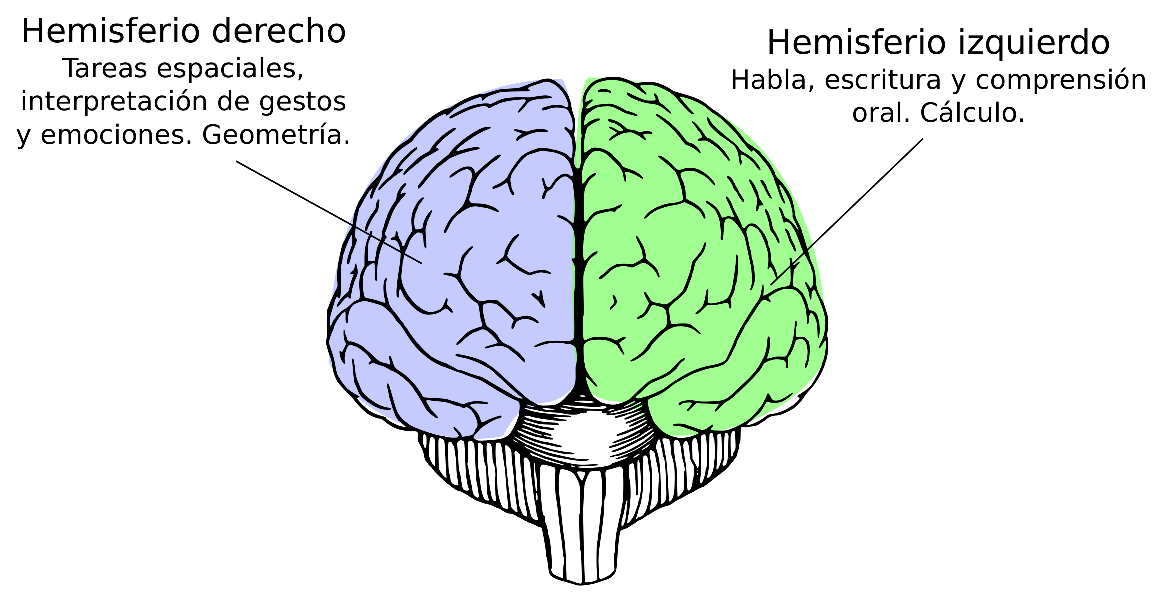
\includegraphics[width=10cm]{images/brain2.eps}
    \caption{Hemisferios cerebrales (vista frontal)}
    \label{hemisferios}
  \end{center}
\end{figure}


\subsection{La corteza cerebral}
\label{sec::corteza-cerebral}

\cite{JohnAllman2000} define ``córtex'' como {\it ``la cubierta externa o corteza de un objeto''}.

\subsubsection{El neocórtex}
\index{neocórtex}
\index{prosencéfalo}\index{mesencéfalo}\index{rombencéfalo}
Como se mencionó en la sección \ref{tubo} cuando se describía el desarrollo del tubo neural, el {\it prosencéfalo} (cerebro anterior), el {\it mesencéfalo} (cerebro medio), y el {\it rombencéfalo} (cerebro posterior) son las partes del cerebro humano durante el comienzo del desarrollo del sistema nervioso central. Durante el desarrollo embrionario el prosencéfalo se divide en {\it diencéfalo} (tálamo e hipotálamo), y {\it telencéfalo} (hemisferios cerebrales).

{\it ''El neocórtex\footnote{También conocido como {\it neocorteza} en la literatura médica española.} es una especialización en el telencéfalo que es paralelo a la formación de la cresta dorsal ventricular en reptiles y aves. El neocórtex es tanto una característica única de mamíferos como son las glándulas mamarias o el martillo y el yunque en el oído medio''}, según \cite{JohnAllman2000}, y {\it ``almacena información acerca de la estructura del medio ambiente a fin de que el mamífero puede fácilmente encontrar alimentos y otros recursos necesarios para su supervivencia''}.

Por otro lado, \cite{Sapolsky} se refiere al {\it neocórtex} como una {\it ``especialización primate''}, terminología que corresponde con la descripción anterior.

\subsubsection{La corteza del cíngulo anterior: emoción, atención y memoria a corto plazo}

Antes de discutir las diferenciaciones anatómicas denominadas lóbulos conviene hablar de la corteza del cíngulo anterior, una zona importante de la corteza cerebral que tradicionalmente se ha considerado parte del sistema límbico\index{sistema límbico}\footnote{Sistema formado por varias estructuras cerebrales que gestionan respuestas fisiológicas ante estímulos emocionales. Está relacionado con la memoria, la atención, los instintos sexuales, las emociones ---placer, miedo, agresividad---, la personalidad y la conducta.}. Desde el punto de vista evolutivo, cabe destacar que la corteza del cíngulo anterior es más antigua que las zonas exteriores de la corteza.


\begin{figure}[h]
  \begin{center}
    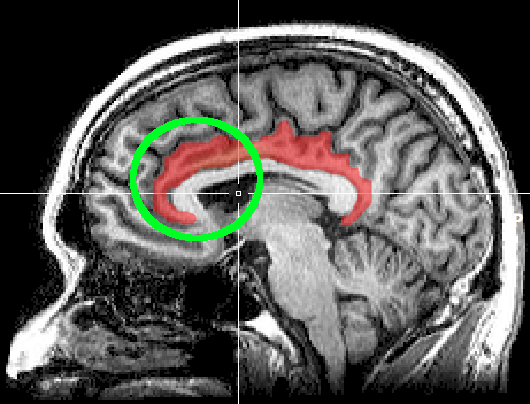
\includegraphics[scale=0.5]{images/cingulo.png}
    \caption{Corteza del cíngulo anterior}
    \label{cingulo}
    % http://upload.wikimedia.org/wikipedia/commons/7/7f/MRI_cingulate_cortex.png
  \end{center}
\end{figure}

La corteza del cíngulo anterior se amolda a la curva exterior del cuerpo calloso, la gruesa banda de fibras nerviosas que conecta los hemisferios izquierdo y derecho del cerebro (ver hemisferios en figura \ref{hemisferios}). El término ``cíngulo'' proviene del latín, y significa cinturón o faja. Este área también es denominada {\it circunvolución cingulada}. \cite{Lindberg.} define ``anterior'' como  {\it ``en relación con o que se encuentra cerca o hacia la cabeza...''}. En la figura \ref{cingulo} la corteza del cíngulo (tanto anterior como posterior) se muestra resaltada, mientras que la parte anterior se encuentra, además, rodeada.

En \cite{Damasio1994} el autor escribe: {\it ``Me gustaría proponer que existe una región particular del cerebro humano donde los sistemas afectados por la emoción / sentimiento, la atención, y la memoria a corto plazo interactúan tan íntimamente que constituyen la fuente de la energía de la acción exterior (movimiento) y la acción interna (pensamiento animación, razonamiento). Esta región manantial es la corteza cingulada anterior, otra pieza del rompecabezas que constituye el sistema límbico\index{sistema límbico}''}. Después continúa diciendo: {\it ``Mi idea acerca de esta región proviene de la observación de un grupo de pacientes con daño en y alrededor de ella. La enfermedad se describe mejor como animación suspendida, mental y externa ---la variedad extrema de un deterioro del razonamiento y de expresión emocional---.''}.

Lo anterior llama la atención sobre un fenómeno interesante que ilustra la función de la corteza cingulada anterior. {\it ``Cuando una apoplejía destruye la corteza motora en el hemisferio izquierdo del cerebro y, como resultado, el paciente tiene parálisis en el lado derecho de la cara''}, comenta \cite{Damasio1994}, {\it ``los músculos no pueden actuar y la boca tiende a ser arrastrada hacia un lado al pedirle al paciente que la abra --- los dientes revelan un aumento de la asimetría---. Sin embargo, cuando el paciente sonríe o se ríe espontáneamente, en respuesta a una observación humorística, sucede algo completamente diferente: la sonrisa es normal, los dos lados de la cara se mueven de forma correcta, y la expresión es natural, nada diferente de la sonrisa habitual pre-parálisis de esa persona. Esto pone de manifiesto que el control motor para una secuencia de movimientos relacionada con las emociones no se encuentra en la misma ubicación que el control de un acto voluntario. El movimiento relacionado con las emociones se desencadena en otras zonas del cerebro, incluso si los músculos objetivos del movimiento son los mismos.''}

Para aclarar que la expresión emocional tiene su origen, \cite{Damasio1994} escribe: {\it ``Si usted estudia a un paciente en el que un golpe ha dañado la corteza cingulada anterior en el hemisferio izquierdo, verá exactamente el resultado opuesto en reposo o en movimiento relacionado con las emociones, la cara es asimétrica, menos móvil en el lado derecho que en el izquierdo. Pero si el paciente trata de contraer los músculos de la cara deliberadamente, los movimientos se llevan a cabo normalmente y vuelve la simetría. La emoción está relacionada con el movimiento, entonces, se controla desde la región cingulada anterior.''}

La corteza cingulada anterior puede desempeñar un papel importante en los lazos entre padres e hijos.

\subsubsection{Los lóbulos cerebrales}
\label{sec:lobulos}
La diferenciación cerebral en ``lóbulos'' se utiliza para indicar la posición relativa de las estructuras cerebrales. Por ejemplo, la amígdala se encuentra dentro de los lóbulos temporales. Es importante recordar que un lóbulo no funciona independientemente, no son unidades autónomas, sino que son meramente una referencia anatómica. \cite{Damasio1994} señala que {\it ``en un sólo segundo el cerebro produce millones de patrones de activación a través de una gran variedad de circuitos distribuidos en varias regiones del cerebro''}.

Si nos centramos en cualquiera de los hemisferios cerebrales por separado, encontramos una nueva división de funcionalidad: los lóbulos cerebrales (figura \ref{lobulos}):

\begin{figure}[h]
  \begin{center}
    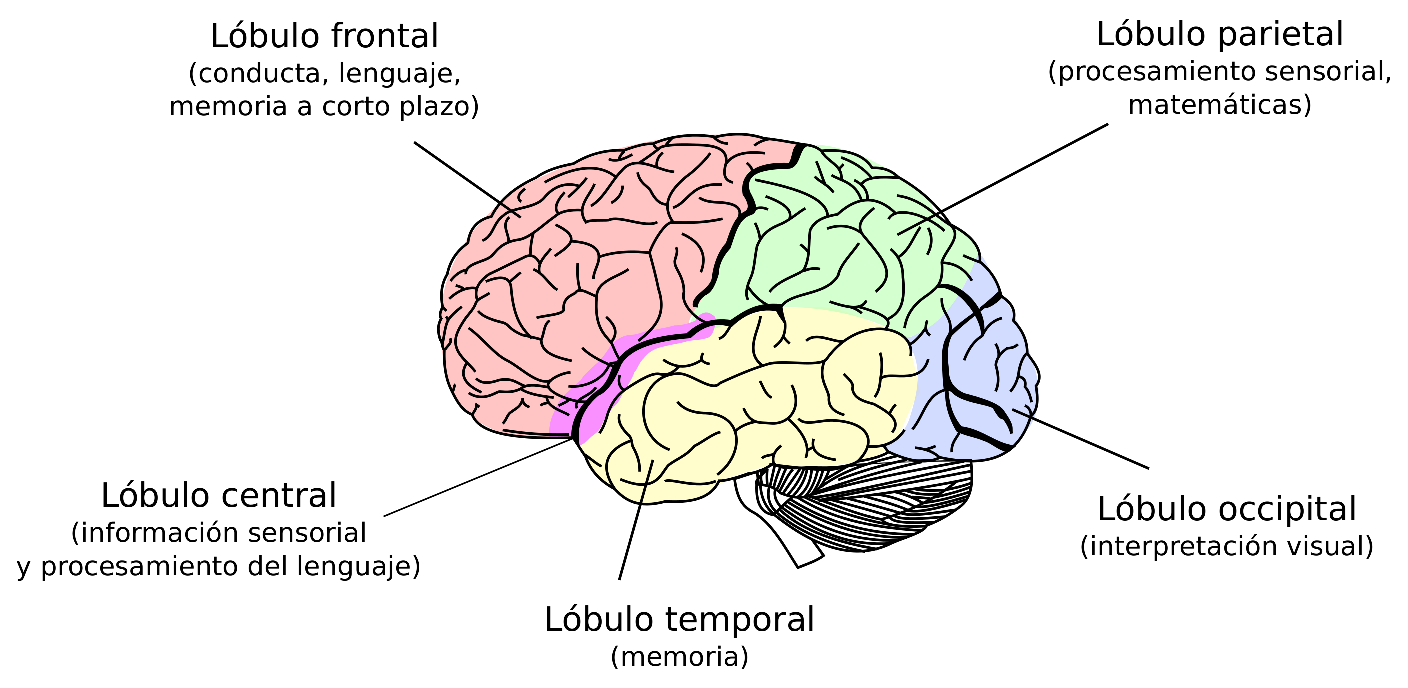
\includegraphics[width=14cm]{images/brain.eps}
    \caption{Lóbulos cerebrales}
    \label{lobulos}
  \end{center}
\end{figure}



\begin{itemize}
\item {\bf Lóbulo frontal}

  Está involucrado en la planificación y priorización de tareas. Según \cite{Restak1995}: {\it ``El lóbulo frontal constituye el 50\% de cada hemisferio cerebral de los seres humanos. Es el encargado de iniciar cualquier actividad motriz, como el habla. Se subdivide en el lóbulo prefrontal ---que integra personalidad con emociones--- y la corteza motora ---que transforma los pensamientos en acciones---.}

\item {\bf Lóbulo temporal}

Contiene un área sensorial relacionada con la audición. Ubicado dentro de cada lóbulo temporal se encuentran la amígdala y el hipocampo, que están, tal como se describe en \cite{Restak1995}, {\it ``implicados en el aprendizaje, la memoria, la experiencia y la expresión de la emoción''}. Una porción del lóbulo temporal, llamada la {\it corteza entorrinal}, conecta las señales corticales de entrada con el hipocampo. {\it ``Las fibras de los cuatro lóbulos, junto con fibras de asociación que unen éstas entre sí, convergen en la región del hipocampo''}, dice \cite{Restak1995}. En \cite{JohnAllman2000} se señala que la amígdala ---tan importante para el procesamiento emocional--- también recibe la entrada de un área cortical en el lóbulo temporal llamada {\it corteza visual inferotemporal}, que es {\it ``más amplia en gran medida en los primates superiores''}. \cite{JohnAllman2000} comenta, además, que {\it ``Charles Goss, Robert Desimone, Rolls Edmund y David Perrett entre otros, han demostrado que las neuronas de la corteza inferotemporal son especialmente sensibles a las imágenes de los rostros''}. \index{córtex/corteza!inferotemporal}


\item {\bf Lóbulo occipital}

Incluye sofisticados mapas topográficos con complejas interconexiones, necesarias para el procesamiento visual y, acorde con \cite{Lindberg.}, tiene {\it ``la forma de una pirámide de 3 lados''}. \cite{MerckCo.} explica que, además de procesar e interpretar la visión, las áreas corticales en el lóbulo occipital permiten al ser humano mantener memorias visuales e integrar percepciones visuales con la información espacial procedente de los lóbulos parietales adyacentes. Si una lesión en la cabeza daña los lóbulos occipitales, en ocasiones se produce lo que se conoce como {\it agnosia visual} ---definida por \cite{MerckCo.} como la {\it ``pérdida de la capacidad de asociar objetos con su habitual papel o función''}---. Con suficiente daño en el lóbulo occipital, {\it ``la gente no puede reconocer caras familiares u objetos comunes, como una cuchara o un lápiz, a pesar de que puede ver estas cosas''}, según se explica en \cite{MerckCo.}.

\item {\bf Lóbulo parietal}

Contiene un área que procesa las sensaciones corporales, llamada {\it corteza somatosensorial}. {\it ``El lóbulo parietal es la estación receptora de la información sensorial desde el lado opuesto del cuerpo y es responsable de la integración de lo que se ve con lo que se siente a través de una red de fibras de asociación''}, explica \cite{Restak1995}.

\item {\bf Lóbulo central o ínsula}

Se encuentra situado {\it ``en el centro del hemisferio cerebral, enterrado entre la unión de los lóbulos frontal y temporal''}, acorde con \cite{Lindberg.}. Según \cite{MerckCo.}, además, la ínsula integra el procesamiento de la información sensorial y autonómica. Involucrado en ciertas funciones del lenguaje, su deterioro puede derivar en la {\it afasia}\index{afasia}, enfermedad que supone la pérdida de capacidad de producir o comprender el lenguaje, tanto hablado como escrito.

\end{itemize}


\subsubsection{La corteza frontal}

\index{neurona!piramidal}

La figura \ref{piramidal} muestra una neurona piramidal, que es común en la corteza prefrontal. La corteza frontal ayuda a centrarse en lo que una tarea es ahora. Los pacientes que sufren demencia en las primeras etapas son incapaces de mantenerse en una tarea concreta, y tienden a volver a tareas anteriores. Sapolsky demostró esta idea con un sencillo experimento consistente en solicitar a pacientes con esta enfermedad que dijeran los meses del año, y después pedirles que contaran hacia atrás a partir 20. El resultado fue que durante la cuenta atrás, los pacientes pasaban a enumerar meses del año, mostrando una imposibilidad para mantener la tarea en la que se encontraban. Esta disfunción se conoce como {\it perseverancia e intrusión} (reversión a una tarea anterior).

\begin{figure}[h]
  \begin{center}
    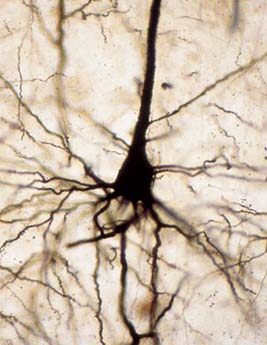
\includegraphics[width=6cm]{images/piramidal.jpg}
    %http://www.kalipedia.com/kalipediamedia/cienciasnaturales/media/200704/17/delavida/20070417klpcnavid_266.Ies.SCO.jpg
    \caption{Neurona piramidal}
    \label{piramidal}
  \end{center}
\end{figure}

{\it ``La corteza frontal está involucrada en el control ejecutivo, sensación de gratificación y planificación a largo plazo''}, explica \cite{Sapolsky2004}. {\it ``Lo hace enviando proyecciones inhibitorias en el sistema límbico\index{sistema límbico}, sistema cerebral involucrado en la emoción y la impulsividad. Además, la corteza frontal resiste entradas estimulantes del sistema límbico\index{sistema límbico}, ignorando tentadores susurros límbicas como \guillemotleft No estudie para el examen, salga a dar una vuelta\guillemotright''}. En el mismo texto se añade que cuando la corteza frontal es destruida, los pacientes sufren deshinibición sexual, agresividad, etc.

Como apunte curioso, en \cite{Johnson2005} se explica cómo si su cerebro se ve dañado en un accidente o derrame cerebral, puede parecer que tiene dañados los lóbulos frontales, incluso cuando los lóbulos frontales permanecen intactos. {\it ``La gente siempre piensa en los lóbulos frontales debido a que son la última estructura en evolucionar, y por lo tanto la más delicada, mientras que las estructuras más antiguas son increíblemente robustas''}. Pero el neuropsicólogo Elkhonon Goldberg, sigue explicando el texto, presentó una teoría diferente: {\it ``Él piensa que, si bien los lóbulos frontales pueden ser más frágiles, hay otro factor en juego, y es que todas las otras partes del cerebro están conectadas a ellos. Al dañar cualquier parte del cerebro, la entrada a los lóbulos frontales se ve alterada, y un cambio en la entrada produce un cambio en la salida. Si los lóbulos frontales no están recibiendo la entrada correcta, es lógico que no produzcan el resultado correcto, aunque estructuralmente estén en perfecto estado. Así que todo el daño cerebral termina pareciéndose a daño en el lóbulo frontal.''}.

{\it ``En los primates, el lóbulo frontal tiene un papel importante en el establecimiento de prioridades y la planificación''}, explica \cite{JohnAllman2000}, {\it ``En particular, la superficie inferior del lóbulo frontal, la denominada corteza orbital-frontal, es especialmente importante para estas funciones''}. La ubicación de la corteza orbital-frontal puede apreciarse en la figura \ref{orbital-frontal}. Cabe destacar que en la literatura médica también se suele utilizar el término {\it región ventromedial del lóbulo frontal} para referirse a la región orbital-frontal.

\begin{figure}[h]
  \begin{center}
    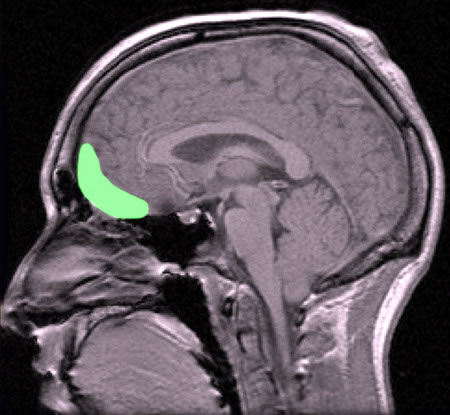
\includegraphics[width=9cm]{images/orbital-frontal.jpg}
    % http://www.blogseitb.com/cienciayhumanismo/wp-content/uploads/2012/10/Orbital-prefrontal-cortex.jpg
    \caption{Corteza orbital-frontal}
    \label{orbital-frontal}
  \end{center}
\end{figure}



\subsubsection{Las áreas de Brodmann}

Según se afirma en \cite{InstituteofNeurosciencesMentalHealth} {\it ``La arquitectura celular difiere suficientemente de una parte del neocórtex a otra como para ser utilizada como un criterio para definir las áreas corticales funcionalmente diferentes''}. Con esa observación, el anatomista alemán Korbinian Brodmann elaboró un mapa de el cerebro basado en las diferencias en la arquitectura celular de las diversas partes de la corteza, asignando a cada parte de la corteza un número del 1 al 52 (ver figura \ref{brodmann}). Respecto a esta división, \cite{InstituteofNeurosciencesMentalHealth} dice: {\it ``La intuición de Brodmann, cuya exactitud ha sido confirmada en muchas ocasiones, afirma que una estructura anatómica particular corresponde a una función en particular. Por ejemplo, el área de Brodmann 17 (que recibe información de un núcleo del tálamo que se conecta a la retina) resulta que corresponde exactamente con la corteza visual primaria.''}. \index{neocórtex}

\begin{figure}[h]
  \begin{center}
    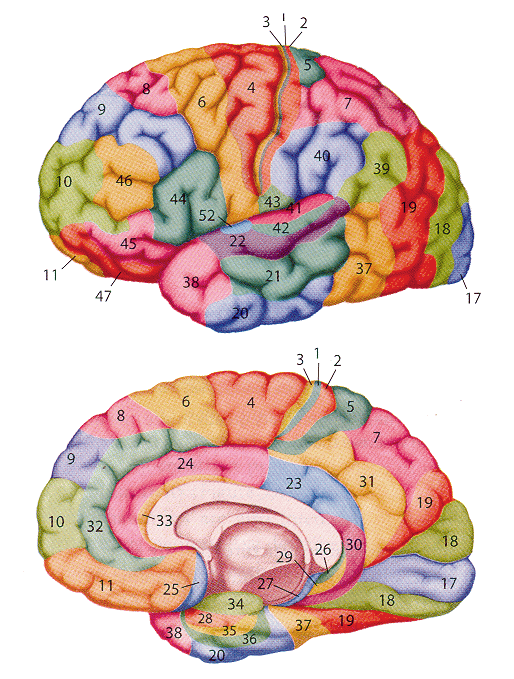
\includegraphics[width=12cm]{images/brodmann-areas.png}
    % http://www.mrc-cbu.cam.ac.uk/people/jessica.grahn/neuroanatomy.html
    \caption{Áreas de Brodmann}
    \label{brodmann}
  \end{center}
\end{figure}


En la figura \ref{brodmann}, {\it la corteza motora primaria} se corresponde con el área 4. El neurocirujano Wilder Penfield Graves (1891-1976) exploró esta región mientras trataba a pacientes con epilepsia severa en Montreal. El objetivo de Penfield era destruir las células nerviosas responsables de la crisis. Mientras el paciente se encontraba bajo el efecto de anestesia local, Penfield estimuló el cerebro con sondas eléctricas, observado las respuestas de los pacientes. Lo hizo para identificar las áreas que requieren cirugía y evitar las áreas vitales que no deben ser destruidas. Al hacer esto, se observó que la estimulación de ciertas áreas de la corteza cerebral desencadenaba contracciones musculares muy localizadas en el lado opuesto del cuerpo. La conclusión fue que las áreas de la corteza asignadas a las diferentes partes del cuerpo {\it ``no son proporcionales a su tamaño, sino más bien a la complejidad de los movimientos que puede realizar. Por lo tanto, las áreas de la mano y cara son especialmente grandes en comparación con las del resto del cuerpo, lo cual no es sorprendente, ya que la velocidad y la destreza de la mano humana y los movimientos de la boca son precisamente los que nos dan dos de nuestras facultades más distintivamente humanas: la capacidad de utilizar las herramientas y la capacidad de hablar.''}.

En \cite{JohnAllman2000} se cita el trabajo de Hughlings Jackson en la determinación de cómo el cerebro controla el movimiento muscular. En la observación de que los pacientes epilépticos en ocasiones sufren crisis convulsivas centradas en un lugar particular en el cuerpo, Jackson {\it ``llegó a la conclusión de que los músculos se representan en el cerebro en un lugar determinado, que dedujo encontrarse en algún lugar de la corteza cerebral o en una estructura cercana llamada cuerpo estriado. Esta teoría fue un cambio radical de la opinión clínica predominante de la época, que era que las crisis epilépticas eran causadas por una alteración en el nivel más bajo del tronco cerebral''}. En el mismo texto puede leerse: {\it ``En 1870, la predicción topográfica de Hughlings Jackson fue confirmada por los médicos alemanes Fritsch y Gustav Eduard Hitzig, quienes descubrieron la corteza motora mediante la estimulación de la superficie del cerebro en perros con débiles corrientes eléctricas y la observación de los movimientos discretos del cuerpo''}. \index{cuerpo estriado}

\index{neocórtex} \cite{JohnAllman2000} explica que las observaciones de Jackson {\it ``se refieren a tres propiedades fundamentales del neocórtex. La primera es que contiene mapas topográficos, la segunda es que las partes más usadas de esos mapas tienen una representación mayor, y la tercera que el neocórtex tiene un papel clave en la génesis de la epilepsia''}. Después continúa diciendo: {\it ``El circuito cortical es muy plástico, ya que puede cambiar su organización funcional en respuesta a la experiencia, y es crucial para la formación de la memoria''}. Esta cualidad plástica del cerebro es la que la literatura médica denomina {\it neuroplasticidad}, concepto que se verá más adelante. \index{neuroplasticidad}

En la figura \ref{brodmann}, las áreas 1, 2 y 3 representan la {\it corteza somatosensorial}, otra especie de mapa topográfico. Si un amigo le hace cosquillas, hay unas zonas muy concretas de la corteza cerebral que se ven activadas. El mapeo somatosensorial permite conocer, monitorizando la actividad cerebral, qué lugar de su cuerpo recibió las cosquillas. En \cite{JohnAllman2000} se explica cómo se descubrieron esos mapas topográficos: {\it ``Con el desarrollo de los amplificadores electrónicos y los osciloscopios de la década de 1930 fue posible registrar la actividad eléctrica de la corteza cerebral. Edgar Douglas Adrian, Woolsey Clinton, entre otros, descubrieron que la región adyacente a la corteza motora se activa eléctricamente por la estimulación mecánica de la superficie del cuerpo; a esa región la llamaron corteza somatosensorial, del griego} soma, {\it que significa} cuerpo. {\it Al registrar actividad en un sitio particular de la corteza somatosensorial, fueron capaces de trazar un campo receptivo en la superficie del cuerpo que activó ese sitio. Con un proceso sistemático encontraron una correspondencia punto a punto en la superficie cortical, por lo que fueron capaces de determinar la representación de la superficie del cuerpo en la corteza somatosensorial''}.

\cite{JohnAllman2000} desarrolla la idea de cómo mediante el uso de grabaciones de microelectrodos, Michael Merzenich, Jon Kaas, y sus colaboradores fueron capaces de confirmar que hay por lo menos cuatro mapas de la superficie del cuerpo en la corteza somatosensorial de los monos. Al igual que los mapas de la corteza motora, los de la corteza somatosensorial en los primates muestran un fuerte énfasis en la mano y la cara, lo que indica la existencia de mayor sensibilidad en las zonas de la mano, los labios y la lengua, que están conectadas a áreas mucho más grandes de la corteza que  las zonas menos sensibles del cuerpo. Al igual que con la corteza motora, los mapas corticales somatosensoriales son plásticos y la representación cortical está más expandida para las partes del cuerpo que son muy usadas. La distinción entre la corteza somatosensorial y la corteza motora no es absoluta. La corteza motora tiene algunas funciones sensoriales y viceversa.

Con respecto al papel de la experiencia en la determinación de las representaciones corticales, \cite{JohnAllman2000} escribe: 

\begin{quote}
  {\it ``Experimentos funcionales realizados en sujetos humanos han demostrado que la representación cerebral de la mano tiene mayor expansión, como resultado de la realización de movimientos complejos de los dedos. La expansión de la representación de la mano puede ser observada tras un corto plazo de capacitación, pero es más notable en los lectores de Braille y en los músicos que tocan instrumentos de cuerda. Estos resultados demuestran el papel de la experiencia: \textit{\textbf{cuanto más fino es el grado de control y el uso de un músculo, mayor será la expansión de su representación en la corteza cerebral}}''}.  
\end{quote}

De nuevo estamos aproximándonos al concepto de {\it neuroplasticidad}, que será desarrollado en la sección \ref{neuroplasticidad}. \index{neuroplasticidad}


\subsubsection{Mapas retinotópicos}

En las áreas del cerebro dedicadas a la vista, los mapas cerebrales son denominados {\it retinotópicos}, puesto que reflejan la topografía de la retina ---la capa de neuronas activadas por la luz que recubren la parte posterior del ojo---. La circuitería visual en la corteza cerebral humana contiene varias docenas de mapas retinotópicos diferentes, cada uno dedicado a analizar el flujo de entrada visual de una forma concreta. La corteza visual primaria ---área 17 de Brodmann (figura \ref{brodmann})--- es el principal receptor de impulsos provenientes de la parte visual del tálamo. Cabe destacar que las áreas visuales además extraen características tales como el color, el movimiento y la forma.

Gran parte del procesamiento visual del cerebro tiene lugar en el lóbulo occipital. Atendiendo a la figura \ref{brodmann}, las áreas dedicadas a esta tarea son la 17, 18, 19, 20 y 21. El área 17 de Brodmann es la corteza visual primaria (V1). El área 18 representa la corteza visual secundaria (V2) y el área 19 la corteza visual asociativa (V3). Cada una de estas áreas constituye un mapa retinotópico. Como se mencionó en el apartado \ref{lobulos}, las áreas de Brodmann 20 y 21 forman parte del lóbulo temporal, y representan la corteza visual inferotemporal, que incluye neuronas sensibles a las imágenes de rostros y envía información visual a la amígdala. \index{córtex/corteza!inferotemporal} \index{córtex/corteza!visual primaria} \index{córtex/corteza!visual secundaria} \index{córtex/corteza!visual asociativa}

En \cite{JohnAllman2000} se detalla cómo la corteza visual primaria (V1) se asignó inicialmente:

\begin{quote}
{\it ``En la guerra entre Rusia y Japón de 1905, muchos soldados japoneses sufrieron heridas de bala en la parte posterior de su cerebro. Debido a la velocidad de salida más alta y el tamaño más pequeño de las balas desarrolladas en el siglo XIX, estas armas tendían a producir lesiones cerebrales más localizadas que las que fueron infringidas en guerras anteriores, lo que mejoró la atención de los heridos y dio lugar a mayores tasas de supervivencia. Muchos de los soldados heridos fueron cegados en parte por estas lesiones, por lo que el oftalmólog Tatsuji Inouye trabajó para el gobierno japonés para evaluar el alcance de su ceguera como un medio para determinar sus beneficios de pensión. Inouye descubrió que la parte del campo visual en el que estos soldados habían quedado ciegos correspondía a la localización de las lesiones cerebrales producidas por los orificios de entrada y salida de la bala. Mediante la combinación del déficit visual de diferentes soldados pudo deducir la organización topográfica de la corteza visual primaria. Inouye reveló que había mucha más corteza dedicada a la representación de la parte central de la retina que a la periferia. Esta es la parte de la retina con mayor agudeza, y es nuestro medio más importante para obtener información del entorno ---y la parte que el lector está empleando en este instante al leer este libro---. El mapa de la corteza visual primaria de Inouye ha sido confirmado por las técnicas modernas de extracción de imágenes cerebrales.''}
\end{quote}

En \cite{Restak1994} se proporciona un ejemplo de cómo el daño a un área del cerebro, en sólo un hemisferio, puede cambiar dramáticamente la forma en que percibimos el mundo. El autor discute cómo Michael Gazzaniga llevó a cabo un experimento que involucró a un sujeto que había perdido la parte izquierda del campo visual a causa de daño cerebral en el área visual del lado derecho de su cerebro: {\it ``Se les pidió que se imaginara a sí mismo mirando hacia California desde Nueva York, y que nombrara los estados que encontraba en medio. Nombró sólo diez estados, todos ellos situados a la derecha de su punto de vista imaginario. Omitió a los estados a la izquierda, que corresponden al campo visual dañado por su lesión cerebral derecha. Lo que no podía ver en el mundo real como resultado de su lesión cerebral, tampoco era capaz de verlo en la imagen espacial de su imaginación''}.

Con el fin de diferenciar la complejidad de las áreas de la corteza visual, en \cite{JohnAllman2000} se citan las diferencias en la corteza visual que distinguen a los primeros mamíferos de los primates y los seres humanos: {\it ``Las zarigüeyas y los erizos, que en muchos aspectos se parecen a los primeros mamíferos que vivieron hace más de 60 millones de años, han limitado su capacidad visual a un pequeño número de las áreas corticales visuales. En los mamíferos, los mapas corticales de la retina son relativamente uniformes en cuanto a la cantidad de espacio cortical dedicado a la parte más central del campo visual, en general en estos animales no es mucho mayor que la corteza dedicada a las partes más periféricas del campo visual. Por el contrario, los primates tienen extremadamente bien desarrolladas las capacidades visuales y tienen un gran número de mapas corticales dedicados a la percepción visual y la memoria. Dentro de la mayoría de estos mapas hay un fuerte énfasis de la representación de la parte central del campo visual y una representación mucho más pequeña de las partes periféricas de la campo visual''}.

\subsection{Estructuras subcorticales. El estrés, las emociones y la enfermedad mental}
\label{sec::estructuras-subcorticales}
% Esta sección es importante. En ella hay un apartado de como el entrenamiento altera el cerebro

En esta sección se estudiarán las principales estructuras subcorticales del cerebro de los mamíferos. En \cite{Panksepp1998}, en referencia al procesamiento emocional instintivo que tiene lugar en nuestras estructuras cerebrales subcorticales, se señala la probabilidad de que, {\it ``en un sentido evolutivo, gran parte del potencial de procesamiento de información en la corteza cerebral es de servicio (se trata de servidores automatizados, a menudo inconscientes) a las instrucciones de los impulsos afectivos que gobernaban el comportamiento previo a la evolución cortical''}.

En \cite{Morrison2009} se ofrece una gran descripción de la similitud entre los humanos y los demás mamíferos. Nosotros, los humanos, compartimos las mismos estructuras cerebrales subcorticales con todos los demás mamíferos. Textualmente:


\begin{quote}

{\it Tanto mi gato Buster como yo nos sobresaltamos y gritamos de dolor ante un estímulo doloroso repentino, y nuestras piernas se contraen en respuesta a un golpe en la rótula de la rodilla. La organización neuronal espinal responsable de estas actividades es la misma, tanto en gatos como en seres humanos.

Profundizando en la parte más baja del cerebro, tanto en Buster como en mí, las mismas neuronas controlan las funciones corporales básicas, tales como la regulación de la respiración, la frecuencia cardíaca y los vómitos. Más hacia adelante residen las células nerviosas que regulan los comportamientos de sueño y la vigilia, que son idénticos en los seres humanos y otros mamíferos, y los resultados de una disfunción en dichas zonas provoca problemas similares, como la narcolepsia \index{narcolepsia} y el trastorno de sueño \acs{REM}. En esta región del cerebro, en todos los mamíferos se encuentran las neuronas que contienen el neurotransmisor dopamina, que degeneran en la enfermedad de Parkinson.

En la base de los hemisferios cerebrales se encuentra la \index{amígdala}amígdala, en forma de almendra, que lidia con el temor y la ansiedad, tanto en personas como animales. Los monos y las ratas han contribuido mucho a nuestra comprensión de la amígdala. La corteza cerebral suprayacente es donde todos nosotros los mamíferos analizamos las sensaciones que provienen de la piel, los músculos y las articulaciones a través de la médula espinal, o los ojos y oídos en el caso de la visión y la audición.

Nos alejamos de otros animales, sin embargo, en el gran desarrollo de la parte delantera de nuestra corteza cerebral, los lóbulos frontales, y la mayor proporción de tejido cerebral, llamadas ``áreas de asociación'', que integran la información obtenida de las regiones que reciben directamente la información sensorial. Estas últimas regiones se llaman las ``áreas primarias sensoriales y motoras'', ya que reciben sensaciones puras y dirigen el movimiento del cuerpo. Se encuentran dentro de los lóbulos frontales, a través de los que nosotros los humanos reflexionamos sobre el pasado y nos preparamos para el futuro. Los animales no tienen esta capacidad última. Los animales se prepararse para el futuro de una forma limitada ---por ejemplo, la ardilla piensa en recolectar y enterrar nueces para el invierno---.}

\end{quote}


\subsubsection{El cerebro animal}

En \cite{Johnson2005} se relata el primer encuentro del autor con con el tejido cerebral real. {\it ``El cerebro de cerdo fue un gran shock para mí porque cuando comparamos las estructuras de nivel inferior, como la amígdala, a las mismas estructuras en el cerebro humano no podía ver ninguna diferencia en absoluto. El cerebro de cerdo y el cerebro humano se veían exactamente idénticos. Pero cuando miré a la neocorteza, la diferencia fue enorme. el neocórtex humano es visiblemente más grande y doblado hacia arriba, y cualquiera puede verlo sin necesidad de un microscopio''}.


\begin{figure}[h]
  \begin{center}
    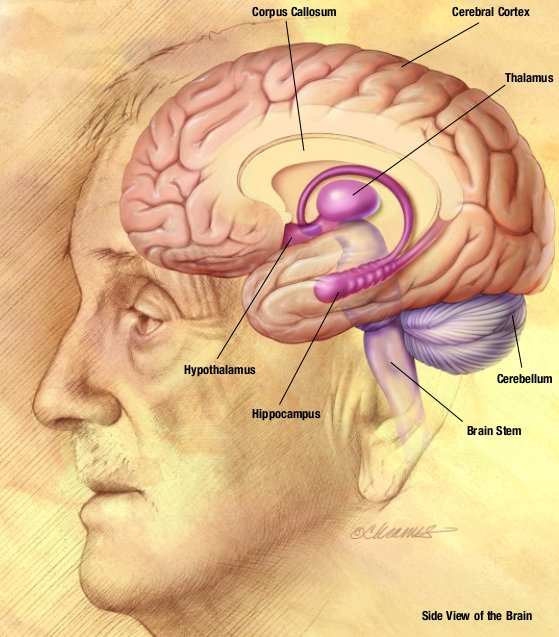
\includegraphics[width=10cm]{images/amigdala.jpg}
    % http://www.neurosciencerus.org/wyHumanBrain.jpg
    \caption{Hipotálamo. Tálamo. Hipocampo. Cerebelo. Cuerpo calloso. Neocórtex. Tallo cerebral}
    \label{fig:amigdala}
  \end{center}
\end{figure}

En la figura \ref{fig:amigdala} se muestra la {\it amígdala}\index{amígdala}, el {\it hipocampo}\index{hipocampo} y el {\it cuerpo calloso}\index{cuerpo calloso}. Debe recordarse que los hemisferios izquierdo y derecho contienen cada una de estas estructuras, que son imágenes especulares el uno de otro.

\subsubsection{La amígdala, el estrés, el \acs{TOC} y el \acs{TEPT}}

\cite{Czerner2001} describe la {\it amígdala}\index{amígdala} como una estructura ``almendrada''. La amígdala se encuentra protegida dentro de cada lóbulo temporal. El lóbulo temporal se encuentra detrás de los templos\index{templo}, de ahí su nombre.

En \cite{Damasio1994} se explica que {\it ``el primer indicio de la relación existente entre la amígdala y las emociones se pueden encontrar en la obra de Heinrich Klüver y Paul Bucy, quienes demostraron que la extirpación quirúrgica de la parte del lóbulo temporal que contiene a la amígdala provoca indiferencia afectiva, entre otros síntomas''}.

Diversas investigaciones demuestran que si la {\it amígdala}\index{amígdala} está dañada, el ser humano pierde la capacidad de discernir las emociones, especialmente el miedo y la ira. Según \cite{JohnAllman2000}, el papel de la amígdala en la percepción de las expresiones faciales {\it ``se mostró claramente en los trabajos de Ralph Adolphs''}. Ralph Adolphs estudió a un paciente que había sufrido un daño bilateral amigdalar sin lesiones significativas en otras partes del cerebro. Aunque este paciente tenía una visión normal y podía percibir rostros, no era capaz de discriminar el contenido emocional de las expresiones faciales negativas del miedo y la ira. Así, todos los rostros le parecían estar sonriendo o mostrando una expresión neutral, incluso los que mostraban un gesto exagerado. El daño a la amígdala\index{amígdala} también afecta a la capacidad para discernir la emoción en el habla. {\it ``Sophie Scott y sus colegas encontraron que la lesión amigdalar también afecta a la capacidad de percibir el contenido emocional de la entonación del habla, a pesar de que su paciente tenía una audición normal. Al igual que con las expresiones faciales en pacientes de Adolphs, las expresiones auditivas del miedo y la ira fueron las más confundidas''}.

El hipocampo y la corteza prefrontal\index{córtex/corteza!prefrontal} se ven reducidos por el estrés, según afirma \cite{Pittenger2008}, mientras que la amígdala\index{amígdala} ve incrementado su tamaño y potenciado su funcionamiento, lo que le permite ser más poderosa con el tiempo ---incluso llegando a ejercer control sobre nuestro razonamiento---. Dicha actividad potenciada puede exacerbar los síntomas de la enfermedad mental, incluyendo el \acs{TOC}.

En \cite{Sapolsky2004} se hace hincapié en que si bien los {\it glucocorticoides}\index{glucorticoides}\footnote{Los {\it glucorticoides} son hormonas de acción contraria a la de la {\it insulina}\index{insulina} en sangre. También actúan sobre el metabolismo intermedio de grasas y proteínas. Los {\it glucocorticoides} producidos por el cuerpo humano son el {\it cortisol}\index{cortisol}, la {\it cortisona}\index{cortisona} y la {\it corticosterona}\index{corticosterona}.} liberados durante episodios de estrés pueden alterar la función del hipocampo y la memoria, los {\it glucocorticoides} mismos incrementan la excitabilidad de la {\it amígdala}\index{amígdala}, permitiendo que las neuronas crezcan más allá de la simple unión entre células.


Especialmente en relación con el \acs{TEPT}, la experiencia es un factor clave. Los neurocientíficos han descubierto que la experiencia moldea la {\it amígdala}\index{amígdala}. Se podría decir que la {\it amígdala} ``aprende'', con el tiempo, el nivel de peligro que debe ser asociado a cada estímulo en particular. En la definición de relevancia incentivo, los autores Vilayanur S. Ramachandran y Lindsay M. Oberman expertos describen el proceso por el cual amígdala puede predecir el peligro. Según \cite{Oberman2006}:

\begin{quote}
{\it ``Cuando una persona ve el mundo, él o ella se enfrenta a una enorme cantidad de información sensorial ---sonidos, olores, etc.---. Después de ser procesada en las áreas sensoriales del cerebro, la información es transmitida a la amígdala\index{amígdala}, que actúa como un portal para el sistema límbico\index{sistema límbico}. La amígdala\index{amígdala} determina la forma en que la persona debe responder emocionalmente: con el miedo (a la vista de un ladrón), la lujuria (al ver a un amante) o indiferencia (cuando se enfrentan a algo trivial). La amígdala envía mensajes al resto del sistema límbico\index{sistema límbico} y, finalmente, alcanza el sistema nervioso autónomo, que prepara al cuerpo para la acción. Si la persona se enfrenta a un ladrón, por ejemplo, su ritmo cardíaco aumenta y su cuerpo comienza a sudar para disipar el calor generado por el esfuerzo muscular. La activación autonómica, a su vez, alimenta al cerebro con información de vuelta, amplificando la respuesta emocional. Con el tiempo, la amígdala\index{amígdala} crea un mapa que detalla el significado emocional de todo en el ambiente del individuo''}.
\end{quote}

En \cite{LeDoux1996} se ofrece un extracto de un informe de Heinrich Klüver y Paul Bucy sobre el comportamiento de un mono tras la extirpación de sus lóbulos temporales ---donde se encuentra la {\it amígdala}\index{amígdala}---. Dicho informe explica cómo el mono no muestra ira ni miedo, y parece incapaz de reconocer objetos:

\begin{quote}
{\it ``El animal, estando hambriento y siendo enfrentado a una variedad de objetos ---un peine, una perilla de baquelita, una semilla de girasol, un tornillo, un palo, un trozo de manzana, una serpiente viva, una pieza de plátano, y una rata viva---, los recoge indiscriminadamente. Lleva cada objeto a la boca, y lo deshecha si no es comestible''}.
\end{quote}

Klüver y Bucy se refieren a este conjunto de síntomas como {\it ``ceguera psíquica''}, dado que los animales tenían una agudeza visual perfecta, pero eran ciegos a la importancia psicológica de los estímulos. Además, \cite{LeDoux1996} explica cómo después de la eliminación de los lóbulos temporales, los monos se convirtieron en {\it ``hipersexuales''}, tratando de copular con otros monos del mismo sexo o con los miembros de otras especies (actividad sexuales rara vez practicada por ``monos normales'').


\subsubsection{Cómo la experiencia afecta al cerebro}

¿Es posible que el entrenamiento pueda crear conexiones neuronales capaces de automatizar comportamientos instintivos? En \cite{Sapolsky} se examina cómo la comunicación entre las neuronas se ve fortalecida como resultado de la experiencia. Sin duda alguna, este punto es clave en el desarrollo de este proyecto, puesto que su pilar fundamental es la posibilidad de mejorar las habilidades mentales mediante cierto tipo de entrenamiento.

Cuando los terminales de las dendritas de las neuronas se estimulan de forma rápida, la comunicación entre las neuronas se ve potenciada {\it ``potenciada''} por ciertos cambios químicos producidos en el contexto neural. Posteriormente, se necesita una menor estimulación para provocar ese mismo nivel de activación neuronal. Esto es así debido a que en el momento en que se percibe una señal eléctrica a través del axón de la neurona, se produce la liberación de los mensajeros químicos llamados {\it neurotransmisores} \index{neurotransmisor} en la sinapsis entre las neuronas, lo que a menudo aumenta la probabilidad de que otras neuronas se dispararen en un especie de reacción en cadena. En otras palabras, el autor afirma que la potencia de activación neuronal se incrementa. Esa potenciación en un tiempo largo es lo que se conoce como {\it ``potenciación a largo plazo''}, y constituye la base para el aprendizaje y la memoria, posiblemente incluso de las formas perjudiciales de aprendizaje, tales como el trastorno de estrés post-traumático (TEPT).

%{\it ``La activación neuronal reconecta el cerebro... anatómicamente el cerebro se forma de nuevo en respuesta a pequeños estímulos nocivos... La activación parece ser un tipo de aprendizaje, pero un aprendizaje que puede ocurrir independientemente de la cognición... la enfermedad, una vez diagnosticada, puede llegar a ser sensible a los estímulos cada vez más pequeños y, con el tiempo, completamente independiente de ellos. El trastorno se vuelve más complejo con el tiempo''}, cita \cite{Kramer1997}.

En \cite{MacLean} el autor teoriza sobre el proceso de activación neuronal: {\it ``Es posible que si un cierto patrón eléctrico de información fuera repetido durante un período prolongado de tiempo, o a intervalos repetidos, en el circuito neuronal, las células nerviosas se sensibilizaran de forma permanente a responder a este patrón particular en algún momento futuro. Tal mecanismo proporciona una variedad de memoria perdurable.''}.

Citando textualmente a \cite{Gallagher}:

\begin{quote}  
{\it Con el tiempo, repetidas experiencias estresantes pueden, literalmente, y no sólo en sentido figurado, alterar el sistema nervioso de las personas. La investigación en animales ha demostrado que cuando a una rata se le da una pequeña descarga no muestra ninguna reacción notable, pero al ser expuesta a factores de estrés tales como la repetición de descargas durante cinco días consecutivos, muestra signos de respuesta al estrés, cuando se expone durante siete u ocho días, la rata tiene un ataque, y a partir de entonces se mantiene alterada y ataca con poca o ninguna provocación. Experimentos de este tipo, por supuesto, no se llevan a cabo con personas, pero Philip Gold y otros neurocientíficos piensan ahora que en los seres humanos, también mediante la activación de una cascada de reacciones químicas, puede producirse un estrés crónico grave, sobre todo en los primeros años de vida, y causar cambios en los genes de manera que se altere la funcionalidad de las células del cerebro de forma permanente. Debido a que las neuronas requieren un tipo particular de entrada para activarse o desactivarse, sólo algunos miles de neuronas, cada una de las cuales está implicado en algún aspecto de la estructura celular o de comunicación, se activan en un momento dado. Cuando una persona de temperamento vulnerable es constantemente bombardeados con estímulos perturbadores, dice Gold, los genes que se activan son los que participan en los componentes celulares de la respuesta al estrés.}
\end{quote}

La neurotransmisión en la amígdala a veces es activada para generar comportamientos impulsados por la {\it dopamina}\index{dopamina}, como conductas orientadas a resolver problemas de control corporal y de confianza. En circunstancias normales, esto puede ser interpretado como un instinto de supervivencia, pero en situaciones de estrés extremo, y especialmente cuando no hay disponible una salida para la energía, estos comportamientos pueden convertirse en obsesiones o compulsiones. \cite{Sapolsky2005} describe cómo los monos liberan dopamina anticipándose a una recompensa alimenticia. Su excitación no alcanza el máximo cuando la comida por fin les llega, sino antes de ese instante. {\it ``Se trata de la anticipación de la recompensa. Se trata de la expectativa y la confianza''}.

% \subsubsection{El hipocampo, la memoria y la depresión}

% \subsubsection{El hipocampo y el TEPT}


% \subsubsection{La amígdala, el hipocampo y la epilepsia}



%% \subsubsection{Hipergrafía y religiosidad}

%% La {\it epilepsia}\index{epilepsia} es una enfermedad crónica caracterizada por uno o varios trastornos neurológicos que predispone al cerebro para generar convulsiones recurrentes. Sin embargo, existe un tipo de epilepsia bastante peculiar: la la epilepsia del lóbulo temporal (\acs{ELT}). La \acs{ELT}, en lugar de provocar crisis convulsivas o pérdida de la consciencia, por lo general produce extraordinarias experiencias subjetivas, entre ellas la {\it autoscopia}\index{autoscopia} ---la sensación de abandonar el cuerpo de uno---. También puede presentarse con {\it hipergrafía}\index{hipergrafía} ---la imperiosa necesidad de escribir---, {\it religiosidad}\index{religiosidad}, o ambas.

%% Como se ha mencionado, la {\it hipergrafía}\index{hipergrafía} es una alteración humana que implica una necesidad imperiosa de escribir. Ese comportamiento podría ser interpretado como algo compulsivo, pero esta clasificación no explica adecuadamente los síntomas. La {\it religiosidad} se puede definir como una devoción excesiva por lo religioso. En algunos casos, como en un ataque epiléptico, el vínculo entre la actividad neuronal y el comportamiento anormal es bien claro. Otros comportamientos, sin embargo, como en la {\it hipergrafía}\index{hipergrafía} y la {\it religiosidad}\index{religiosidad}, no son tan fácilmente atribuibles a la actividad neuronal, ya que a menudo parecen ser racionales. Una persona que sufre de {\it hipergrafía} o {\it religiosidad} a menudo considera su conducta como intencional, sin serlo.

%% En \cite{LaPlante2000} se toma nota de las observaciones de Norman Geschwind, neurólogo del siglo XX. En la evaluación de algunos de sus pacientes epilépticos, Geschwind descubrió que la {\it hipergrafía}\index{hipergrafía} tenía lugar a menudo en los pacientes que atribuían a sus experiencias un significado religioso y moral. La teoría de Geschwind implica que el exceso de actividad en el lóbulo temporal ---recuérdese una vez más que la {\it amígdala}\index{amígdala} y el {\it hipocampo}\index{hipocampo} se encuentran en el lóbulo temporal\index{lóbulo!temporal}--- {\it ``mejora las funciones normales de la emoción y la memoria, haciendo que los pacientes sientan experiencias inusualmente profundas, para atribuir a esas experiencias un significado religioso o moral, y para grabarlas compulsivamente en dibujos o escrituras''}.

% \subsubsection{El tálamo y el TOC}


% \subsubsection{El hipotálamo y la búsqueda}


% \subsubsection{Hipotálamo, el apetito, el apego y la anorexia}

% \section{Los neurotransmisores y las emociones} %% parte 2 de la web
% \label{neurotransmisores}

% \subsection{Introducción a los neurotransmisores}


% \subsection{Los neurotransmisores y la enfermedad}


% \subsection{Conexiones emocionales}


% \subsection{El sistema de búsqueda del cerebro}


% \subsection{Atención, aprendizaje y memoria: Sistema de vigilancia}


% \subsection{Sistemas innatos del cerebro}


% \subsubsection{La rabia}


% \subsubsection{El miedo}


% \subsubsection{La diversión}


% \subsubsection{La cautela}

% \section{El comportamiento innato}% parte 3 de la web
% \label{comportamientoinnato}
% \subsection{Estrés y aislamiento}


% \subsection{Trastorno dismórfico corporal, tricotilomanía, y pellizcos en la piel}

% \subsection{Trastorno obsesivo-compulsivo}


% \label{sec::estres-cronico}


%%%%%%%%%%%%%%%%%%%%%%%%%%%%%%%%%%%%%%%%%%%%%%%%%%%%%%%%%%%%%%%%%%%%%%%%%%%%%%%%


\section{Neuroplasticidad}
\label{neuroplasticidad}

Como se explica en \cite{Statement2012}, diversas investigaciones en el campo de la neurología concluyen que el cerebro humano, en lugar de tratarse de una \emph{``masa de células estática''}, se trata de un sistema dinámico de redes neuronales con gran potencial de crecimiento bajo unas circunstancias favorables. La publicación diferencia esas circunstancias en dos periodos:

\begin{itemize}
\item {\bf Periodo crítico}: Cuando el cerebro del individuo es más sensible a las influencias del entorno.
\item {\bf Periodo sensible}: Cuando el cerebro es menos susceptible a la influencia exterior.
\end{itemize}

Sin embargo, el fin del periodo crítico no implica que el cerebro ``se estanque'' y deje de ser susceptible de verse mejorado, sino que el nivel de neuroplasticidad de esa etapa no será alcanzado fuera de ella. Por tanto, durante el periodo sensible es necesario un mayor esfuerzo para mejorar algún aspecto cerebral que para obtener la misma mejora durante el periodo crítico.

En \cite{Facts2006} se introduce la idea de cómo el \ac{SFC} se relaciona con una reducción de la materia gris cerebral, sirviéndose de diversas técnicas no invasivas de obtención de información cerebral mediante imágenes ---como la \ac{IRM} o la \ac{VBM}---, para explicar después que la plasticidad cerebral permite que algunos pacientes con este problema recuperen cierta funcionalidad de procesamiento cerebral perdida.

El cerebro de un músico es un objetivo de estudio perfecto para analizar la neuroplasticidad: los pianistas, por ejemplo, deben coordinar la producción de hasta 1800 notas por minuto con ambas manos (ver figura \ref{fig::partitura}); la composición musical, además, requiere de la integración de información sensorial y motora, junto a una precisa observación de la ejecución. Estos argumentos son los que presenta \cite{Munte2002} para justificar cómo el cerebro de un músico es un buen ejemplo de neuroplasticidad. En dicho artículo se explica cómo varios años de experiencia musical ---sobre todo cuando los individuos empiezan sus estudios musicales a una edad temprana--- pueden estar relacionados con un aumento en las materias gris y blanca\index{materia!gris}\index{materia!blanca}, así como en el volumen, de las regiones 31, 32, 36, 39 y 41 del cerebro (ver figura \ref{brodmann}).

\begin{figure}[h]
  \begin{center}
    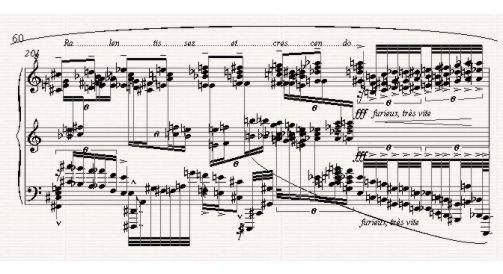
\includegraphics[width=\textwidth]{images/piano.jpg}
    \caption{Ejemplo de partitura de piano compleja, extraída de una pieza de Kaikhosru Shapurji Sorabji}
    \label{fig::partitura}
  \end{center}
\end{figure}


\cite{Melzack2001} relaciona el dolor crónico y patológico con la neuroplasticidad\index{neuroplasticidad}. Para ello estudia el {\it síndrome del miembro fantasma} ---percepción de sensaciones de que un miembro amputado todavía forma parte del cuerpo y funciona correctamente---. Antiguamente se solía pensar que estas sensaciones se debían a que el cerebro seguía recibiendo mensajes de los nervios que originalmente llevaban impulsos desde el miembro amputado. Sin embargo, la creencia actual se basa en que el cerebro sigue conservando un área dedicada a dicho miembro, por lo que el individuo sigue ``sintiéndolo''. Los estímulos sensoriales actúan sobre sistemas neuronales que fueron modificados por entradas anteriores, y su comportamiento y salida están influenciados por la ``memoria'' de esos eventos del pasado. \cite{Melzack2001} relaciona esto con la neuroplasticidad\index{neuroplasticidad} en el sentido en que en la mayoría de casos la sensación del miembro fantasma desaparece, al menos de forma temporal, sometiendo a los individuos a visiones que revelen la no correspondencia entre el miembro real y el percibido.

El estrés crónico ---el cual puede derivar en depresión--- interrumpe la neuroplasticidad de forma temporal, explica \cite{Pittenger2008}, mientras que un tratamiento antidepresivo ofrece el resultado opuesto.

Yendo más lejos, en \cite{May2008} se desarrolla la idea del {\it cambio cualitativo}\index{cambio cualitativo} ---aprendizaje de nuevas tareas--- como principal impulsor de la modificación estructural del cerebro, por encima de la práctica reiterada de un ejercicio conocido. Para ello se estudia el efecto del aprendizaje de juegos malabares por parte de 20 individuos, observando cómo este ejercicio produce una alteración de la materia gris del {\it córtex occipitotemporal}\index{córtex/corteza!occipitotemporal} con tan sólo una semana de entrenamiento.

\subsection{Memoria (Memory)}

\subsubsection{Memoria de trabajo}
\label{sec::memoria-trabajo}
En \cite{Jaeggi2008} se estudia la forma de estimular la memoria de trabajo a lo largo de cuatro experimentos, empleados para mejorar lo que denomina ``{\it inteligencia fluida}''. Ésta es una habilidad compleja humana que posibilita la adaptación del pensamiento a nuevas situaciones o problemas a los que nunca antes nos habíamos enfrentado.

El hecho de mejorar la memoria de trabajo como un medio para conseguir un fin mayor, como el mencionado, pone de manifiesto la importancia de este tipo de memoria, que es empleada en la resolución de problemas o realización de tareas complejas.

La memoria de trabajo también es empleada como medio para conseguir un objetivo diferente ---y más ambicioso si cabe--- en \cite{Olesen2004}. El texto relata como, mediante la estimulación de la memoria de trabajo a través de diversos experimentos, se consigue incrementar la actividad prefrontal y parietal del cerebro. Si recordamos la diferenciación de los lóbulos cerebrales expuesta en la sección \ref{sec:lobulos}, los lóbulos prefrontal\index{lóbulo!frontal} y parietal\index{lóbulo!parietal} albergan el procesamiento de emociones y de la información sensorial, respectivamente.

\subsubsection{Recuerdo espacial (Spatial recall)}

Este aspecto funcional del cerebro se encarga del almacenamiento a largo plazo de representaciones visuales. Una forma elegante de explicar su comportamiento es mediante la creación de un modelo del mismo, como hace \cite{becker}, y la posterior simulación de su comportamiento en entornos complejos. La lectura relata el efecto de daños cerebrales artificiales producidos sobre el modelo, concretamente en lóbulo parietal\index{lóbulo!parietal}, y utilizan sus resultados para la realización de predicciones sobre la representación neural que tiene lugar en el cerebro.

En lineas generales, el modelo consiste en lo siguiente: un {\it parahipocampo}\footnote{Estructura compleja que recubre el hipocampo por su parte inferior. También es denominado {\it circonvolución parahipocámpica}} genera una representación alocéntrica de los objetos a partir de un {\it flujo visual ventral} ---qué es el objeto---, mientras que el lóbulo parietal\index{lóbulo!parietal} interpreta un {\it flujo visual dorsal} para generar una representación egocéntrica ---dónde se encuentra el objeto---. Una conexión bidireccional recurrente entre las regiones egocéntrica y alocéntrica produce la memoria a largo plazo.

Atendiendo al objetivo del presente proyecto, resulta de aún más interés el estudio de \cite{Hirvasoja2004}, donde se analiza el efecto que los videojuegos pueden ejercer sobre las habilidades espaciales. Una de las hipótesis más interesantes del estudio es la existencia de un comportamiento diferente entre sexos ante la estimulación ejercida por los videojuegos. Mediante un experimento en el que algunos individuos son sometidos a la práctica de un juego 3D durante 5 horas seguidas se puede observar, entre otras cosas, que las mujeres presentan una mejora de las habilidades espaciales ligeramente mayor que los hombres.

\subsubsection{Recuerdo cara-nombre (Face-name recall)}

Denominamos {\it recuerdo cara-nombre} a la habilidad cerebral para mantener una correspondencia entre nombres de personas y sus caras. En \cite{Haxby2000} se propone un modelo estructural que explica el sistema neural encargado de esta habilidad, una de las más desarrolladas en los seres humanos frente a otros animales. No obstante, se concluye que la diferenciación fisiológica de los elementos participantes en este comportamiento es algo difusa, dando pie a la realización de otros posibles modelos que lo expliquen.

Por otro lado, \cite{Trinkler2009} muestra algunos resultados experimentales sobre el reconocimiento facial por parte de algunos voluntarios: los individuos son sometidos a la visualización de un conjunto de rostros ---de forma secuencial--- durante unos instantes, para mostrarles otro conjunto diferente (con ciertos rostros en común con el primero) después. Los individuos deben reconocer las caras que han aparecido en ambos conjuntos y las que aparecen en el segundo conjunto y no formaban parte del primero.

El hipocampo\index{hipocampo} es el absoluto protagonista en la asociación cara-nombre.

\subsection{Resolución de problemas (Problem solving)}
\label{sec::problem-solving}

\subsubsection{Aritmética (Arithmetic)}

Centrándonos en los efectos neuroplásticos relacionados con la aritmética, en \cite{Dehaene2004} se explica cómo la realización de cálculos por parte de los seres humanos se ve reflejada en la activación del \acf{SIP}\footnote{Hendidura irregular en la superficie convexa del lóbulo parietal, que marca la división entre los lóbulos parietales\index{lóbulo!parietal} superior e inferior.}. Un estudio adicional que corrobora este hecho descubre que ciertas patologías de esa zona cerebral producen la denominada {\it acalculia}\index{acalculia} ---imposibilidad para la realización de cálculos matemáticos, sencillos o complejos---.

Las propuestas futuras que se realizan en \cite{Dehaene2004} abarcan la comprensión de las homologías y diferencias entre la actividad cerebral de determinados simios y los seres humanos.

\subsubsection{Razonamiento lógico (Logical reasoning)}

El razonamiento lógico tiene lugar principalmente en el lóbulo frontal\index{lóbulo!frontal}, y consiste en la habilidad para combinar procesos cognitivos y la flexibilidad para reconocimiento de patrones, extracción de conclusiones y toma de decisiones. Como recurso de interés para adentrarse en el mundo de la lógica, \cite{JulianIranzo2004} ofrece un manual completo sobre las lógicas de proposiciones y predicados, enfocado al aprendizaje por parte de personas del ámbito de la Ingeniería Informática.

El razonamiento lógico permite, partiendo de uno o más juicios, derivar la validez o falsedad de otro juicio distinto. Para \cite{DeWall2008} {\it ``el sistema de procesamiento consciente y reflexivo es vital para el razonamiento lógico''}. Por tanto, se podría afirmar que el razonamiento lógico es un proceso consciente.

\subsubsection{Razonamiento cuantitativo (Quantitative reasoning)}

Los seres humanos empleamos el razonamiento cuantitativo para realizar estimaciones. Resulta de utilidad para comparar precios de productos y cuotas, valor de impuestos, etc. Especialmente en el mundo empresarial, el razonamiento cuantitativo es empleado para la toma de decisiones de negocio y selección de estrategias.

\subsection{Atención (Attention)}

\subsubsection{Concentración (Focus)}

La concentración no es más que la capacidad para prestar atención a la información pertinente, ignorando distracciones irrelevantes. Resulta de gran importancia en situaciones que impliquen realizar una tarea como la lectura en un entorno ruidoso como una cafetería. La densidad de información que llega a nuestros sentidos es inmensa, por lo que la concentración para desechar cualquier información no relevante es de alta importancia.

En \cite{Bherer2006} se exponen los resultados obtenidos tras un experimento en el que personas jóvenes y mayores son sometidas a un cierto programa de entrenamiento centrado en el control de la atención. Los resultados indican una mejora sustancial en la atención ---gracias a la {\it neuroplasticidad}\index{neuroplasticidad}---, curiosamente equivalente en ambos grupos de edad.

\subsubsection{Campo visual (Visual field)}

El campo visual consiste en el espacio que un individuo puede ver en un momento dado sin mover sus ojos. Implica a la visión periférica y resulta de gran importancia cuando se conduce un vehículo o se practican ciertos deportes. La mejora del campo visual, por tanto, supone un mecanismo muy efectivo para mejorar también nuestro rendimiento llevando a cabo esas actividades.

El campo visual disminuye con la edad, como expone \cite{Ball1988}. Sin embargo, mediante cierto tipo de videojuegos es posible realizar mejoras importantes en esta habilidad, entre otras, tal y como expresa \cite{Green2003} en anteposición a lo que comúnmente es denominado {\it ``aprendizaje perceptivo''}\footnote{Mejora de la respuesta a estímulos mediante una exposición duradera a los mismos}.

\subsection{Velocidad (Speed)}

\subsubsection{Procesamiento de información (Information processing)}

%http://blog.lumosity.com/information-processing/

Esta habilidad mental consiste en la captura e interpretación de la información sensorial que recibimos. Realizar esta tarea de forma rápida nos permite mejores tiempos de respuesta y capacidad de adaptación frente a cambios en nuestro entorno. Una de las tareas cotidianas en las que la velocidad de procesamiento de información adquiere gran importancia es la condución.

{\it ``A medida que el ser humano envejece''}, tal y como explica \cite{Wood2005}, {\it ``el rendimiento de nuestras habilidades funcionales decrece de forma significativa''}, lo que afecta de forma directa a nuestra velocidad de procesamiento de información. No obstante, es en \cite{Karlene2007} donde se muestran resultados claros ---mediante seis estudios diferentes--- del impacto que el entrenamiento cognitivo y produce sobre la velocidad de procesamiento. Curiosamente, además, concluye que {\it ``la edad y la educación tienen un impacto muy pequeño o nulo sobre la ganancia producida por el entrenamiento''}.

\subsubsection{Orientación espacial (Spatial orientation)}

La orientación espacial consiste en encontrar la dirección deseada en movimiento en un entorno físico. Se pone de manifiesto cuando nos desplazamos por una ciudad que no conocemos, así como durante la lectura e interpretación de un mapa. Se trata de una capacidad innata en gran parte, pero que puede mejorarse mediante entrenamiento.

Esta habilidad presenta diferencias entre hombres y mujeres. Sin embargo, \cite{Jing2007} afirma que dichas diferencias desaparecen parcialmente tras la práctica de ciertos ejercicios mediante videojuegos. Por otro lado, \cite{Lynn1994} documenta los efectos del entrenamiento de la orientación espacial mediante videojuegos, así como posibles formas de medir esa mejora ---de gran interés para el proyecto que nos ocupa---.

\subsection{Flexibilidad (Flexibility)}

\subsubsection{Control de impulsos (Response inhibition)}

El control de los impulsos es una habilidad mental humana que nos diferencia del resto de animales. Nos permite priorizar acciones teniendo en mente los objetivos a los que nos enfrentamos, controlando nuestros impulsos animales. En \cite{Zheng2008} se habla del control de impulsos como la {\it ``la función cerebral más evolucionada del ser humano''}.

{\it ``Conocer cómo está implementado este control de impulsos en el cerebro es uno de los mayores problemas de la neurociencia contemporánea''}, afirma \cite{James2009}.

\subsubsection{Planificación (Planning)}

La planificación es la capacidad cerebral que posee el ser humano para priorizar diferentes tareas a lo largo de un periodo de tiempo. Resulta de gran importancia, en combinación con la capacidad para intercambiar el foco de atención entre esas tareas (habilidad que se estudiará a continuación).

\subsubsection{Conmutación de tareas (Task switching)}

La conmutación de tareas supone la adaptación al cambio en el entorno, detectando cuándo y en qué situaciones resulta más beneficioso pasar a realizar otra tarea en lugar de continuar con la que estaba en curso, así como en qué momento volver a la primera tarea. Resulta inmediata la relación de esta habilidad con lo que en computación se conoce como {\it multitarea}\footnote{Característica de los sistemas operativos modernos de permitir que varios procesos sean ejecutados (en apariencia) al mismo tiempo, compartiendo uno o más procesadores.}. Gracias a la conmutación de tareas el ser humano es capaz de cambiar su foco de atención en base a cambios ajenos a él en su contexto.

En relación con la memoria de trabajo (vista en la sección \ref{sec::memoria-trabajo}), en \cite{Klaus2004} se realiza una prueba de significación de la hipótesis de que, con una práctica adecuada, el ser humano es capaz de emplear la memoria de trabajo para ejecutar dos operaciones simultáneas.

\subsubsection{Fluidez verbal (Verbal fluency)}

La fluidez verbal supone el acceso veloz al vocabulario conocido durante una conversación o tarea de escritura. Consiste en el ingenio y la capacidad de intercambio y conexión de palabras, y resulta crucial para la comunicación.

Esa conocida sensación de {\it ``tener una palabra en la punta de la lengua''} está relacionada estrechamente con la fluidez verbal. Depende de multitud de factores, como la edad, cuyo efecto se analiza en \cite{Deborah2004}.

\section{Sistemas de recomendación}

Los sistemas de recomendación, como área de investigación independiente, surgieron a mediados de los noventa. En su fórmula más común, el problema de la recomendación se reduce a {\it la clasificación estimada de elementos que no han sido vistos por el usuario} \cite{adomavicius}. Dicha estimación se basa, entre otra información, en la valoración que el usuario ha hecho de otros elementos relacionados.

Supongamos que $U$ es el conjunto total de usuarios, y $S$ el conjunto de elementos que pueden ser recomendados a cada usuario $u \in U$. Cada elemento $u$ tiene un perfil asociado con información personal como edad o sexo, intereses, etc. Por otro lado, cada elemento o artículo susceptible de ser recomendado, $s \in S$, está definido por un conjunto de características. Llamemos $f$ a la función de utilidad que, para cada usuario $u$ y cada elemento $s$, tiene como valor la utilidad del item $s$ para el usuario $u$ (lo que representaremos como $s_u$):

$$
\begin{array}{rccc}
f: & U \times S & \longrightarrow & \mathbb{R}\\
   & u, s & \longrightarrow & s_u
\end{array}
$$

$f$ estará definida en aquellos puntos en los que conocemos exactamente la valoración que el usuario realiza sobre el artículo ---en el caso de una colección de películas, la valoración puede ser la puntuación que el usuario le da a la película de forma explícita---. El objetivo de un sistema de recomendación es extrapolar la función $f$ a todo el espacio $U \times S$, de forma que se pueda estimar la utilidad que cada elemento $s$ tiene para cada usuario $u$.

Para extrapolar la función $f$ se suelen emplear dos métodos diferentes:

\begin{enumerate}
\item Mediante una heurística
\item Estimando la función de utilidad que optimiza algún criterio (como el menor error cuadrático, por ejemplo)
\end{enumerate}

Una vez calculada la estimación, el elemento $s$ recomendado al usuario $u$ será aquel que mayor valoración tenga según la función $f$. Si llamamos $s'_u$ a la puntuación más alta:

$$
\forall u \in U,\quad s'_u = \max_{s \in S}\ f(u,s)
$$

\subsection{Tipos de sistemas de recomendación}

En \cite{adomavicius} se realiza una clasificación de los sistemas de recomendación en base al tipo de función de utilidad:

\begin{enumerate}

\item {\bf Recomendación basadas en el contenido}

Los artículos o items recomendados al usuario son similares a aquellos a los que el usuario mejor valoró en el pasado. Es decir, la utilidad $f(u,s)$ es estimada en base a las valoraciones $f(u,s_i)$ que el usuario $u$ realizó explícitamente sobre los items $s_i \in S$ similares a $s$.

\item {\bf Recomendación colaborativas}

Los items recomendados al usuario son los que las personas similares a él mejor valoraron en el pasado. Formalmente, la utilidad $f(u,s)$ es estimada en base a las valoraciones $f(u_i,s)$ realizadas por los usuarios $u_i \in U$ similares a $u$.
\end{enumerate}

Además de los dos métodos anteriores, existe la posibilidad de seguir un {\bf enfoque híbrido}, como una combinación de los dos anteriores, para superar las limitaciones de ambos. Existen diferentes formas de realizar dicha combinación:

\begin{itemize}
\item Implementar los métodos basado en contenido y colaborativo por separado y combinar sus estimaciones.
\item Implementar algunas características de la recomendación basada en contenido sobre un sistema de recomendación colaborativa.
\item Implementar algunas características de la recomendación colaborativa en un sistema de recomendación basada en contenido.
\item Implementar un sistema global basado en las características de ambos.
\end{itemize}

A la vista de lo anterior, resulta evidente la necesidad de definir una función de similitud entre artículos (para el caso 1) y una función de similitud entre usuarios (para el caso 2). Dichas funciones dependerán del contexto en el que el sistema de recomendación se enmarque, es decir, de la información que haya disponible de los artículos y usuarios.

Por otro lado, en \cite{burke} se contemplan tres métodos de recomendación además de los ya mencionados:

\begin{enumerate}
\setcounter{enumi}{2}

\item {\bf Recomendación demográfica}

Categoriza a los usuarios en clases demográficas, en base a las características personales. En lugar de utilizar valoraciones pasadas (como los métodos anteriormente vistos), utiliza dichas clases para realizar las estimaciones de utilidad.

\item {\bf Recomendación basada en utilidad}

La recomendación se basa en el cálculo de una función de utilidad de cada item para cada usuario, pero teniendo en cuenta aspectos dinámicos ---como la disponibilidad de un producto en un momento dado, en el caso de una tienda---.

\item {\bf Recomendación basada en conocimiento}

Trata de realizar inferencias sobre las necesidades y preferencias de los usuarios, basándose en un {\it conocimiento funcional} \cite{burke}: información sobre cómo un determinado artículo coincide con una necesidad del usuario. El perfil de usuario debe contener algún tipo de estructura de conocimiento que soporte esta inferencia. En el caso sencillo de un buscador, esa información del usuario puede ser símplemente la búsqueda que ha realizado.

\end{enumerate}

En la tabla \ref{table::recomendacion} se muestra un resumen de los diferentes métodos de recomendación expuestos.

\begin{table}
  \label{table::recomendacion}
  \begin{center}
  \begin{tabular}{|l||l|l|l|}
    \hline
    \tabheadformat
    \tabhead{Método} & \tabhead{Fundamento} & \tabhead{Entrada} & \tabhead{Proceso} \\
    \hline
    \hline
    Basada en & a & a & a\\
    contenido & a & a & a\\
    \hline
    Colaborativa & a & a & a\\
    \hline
    Demográfica & a & a & a\\
    \hline
    Basada en & a & a & a\\
     utilidad & a & a & a\\
    \hline
    Basada en & a & a & a\\
 conocimiento & a & a & a\\
    \hline
  \end{tabular}
  \caption{Tipos de recomendación}
  \end{center}
\end{table}
